\documentclass[paper=a4, fontsize=11pt]{scrartcl}	% 

\usepackage[brazil]{babel}
\usepackage[utf8]{inputenc}
\usepackage[protrusion=true,expansion=true]{microtype}				% Better typography
\usepackage{amsmath,amsfonts,amsthm}										% Math packages
\usepackage[pdftex]{graphicx}														% Enable pdflatex
%\usepackage{color,transparent}													% If you use color and/or transparency
\usepackage[hang, small,labelfont=bf,up,textfont=it,up]{caption}	% Custom captions under/above floats
\usepackage{epstopdf}																	% Converts .eps to .pdf
\usepackage{subfig}																		% Subfigures
\usepackage{booktabs}																	% Nicer tables
\usepackage{hyperref}

%%% Advanced verbatim environment
\usepackage{verbatim}
\usepackage{fancyvrb}
\DefineShortVerb{\|}								% delimiter to display inline verbatim text


%%% Custom sectioning (sectsty package)
\usepackage{sectsty}								% Custom sectioning (see below)
\allsectionsfont{%									% Change font of al section commands
	\usefont{OT1}{bch}{b}{n}%					% bch-b-n: CharterBT-Bold font
%	\hspace{15pt}%									% Uncomment for indentation
	}

\sectionfont{%										% Change font of \section command
	\usefont{OT1}{bch}{b}{n}%					% bch-b-n: CharterBT-Bold font
	\sectionrule{0pt}{0pt}{-5pt}{0.8pt}%	% Horizontal rule below section
	}


%%% Custom headers/footers (fancyhdr package)
\usepackage{fancyhdr}
\pagestyle{fancyplain}
\fancyhead{}														% No page header
\fancyfoot[C]{\thepage}										% Pagenumbering at center of footer
\fancyfoot[R]{\small \texttt{Monografia}}	% You can remove/edit this line 
\renewcommand{\headrulewidth}{0pt}				% Remove header underlines
\renewcommand{\footrulewidth}{0pt}				% Remove footer underlines
\setlength{\headheight}{13.6pt}

%%% Equation and float numbering
\numberwithin{equation}{section}															% Equationnumbering: section.eq#
\numberwithin{figure}{section}																% Figurenumbering: section.fig#
\numberwithin{table}{section}																% Tablenumbering: section.tab#


%%% Title	
\title{ \vspace{-1in} 	\usefont{OT1}{bch}{b}{n}
		\huge \strut Organização de Video-Games - SNES \strut \\
		\Large \bfseries \strut \strut
}
\author{ 									\usefont{OT1}{bch}{m}{n}
        Alessandro Palmeira \hspace{7.37cm} 6850476
        \\		\usefont{OT1}{bch}{m}{n}
        João Marco Maciel da Silva  \hspace{5.7cm} 7577598
        \\		\usefont{OT1}{bch}{m}{n}
        \\Universidade de São Paulo\\	\usefont{OT1}{bch}{m}{n}
        Instituto de Matemática e Estatística\\
        \usefont{OT1}{bch}{m}{n}
                MAC 0412 - Organização de Computadores
}
\date{}

%%% Begin document
\begin{document}
\maketitle
\section{Introdução}
Vídeo-games fizeram parte da história da computação desde o início e, particularmente, foram o primeiro contato entre os autores e o universo dos computadores. O Super Nintendo Entertainment System - SNES, foi escolhido para essa pesquisa principalmente pelos seguintes fatores:
\begin{itemize}
  \item{Sistema relativamente simples, composto basicamente por circuitos integrados disponíveis no mercado}
  \item{Sistema complexo o suficiente para ter um ótimo valor educacional}
  \item{Valor sentimental e nostálgico para os autores}
\end{itemize}
Primeiramente faremos um breve resumo da história dos Vídeo-Games para delinearmos um contexto histórico. Em seguida mergulharemos mais à fundo nos componentes e no conjunto do SNES, também conhecido como Super Famicom (Family Computer).

\section{História dos Vídeo Games}
A história dos Vídeo-Games pode ser dividida em 9 periodos.
\subsection{Pré-História}
A pré-história dos Vídeo-games remete ao período da decada de 40, quando, em 1947, \textit{Thomas T. Goldsmith }e \textit{Estle Ray Mann }patentearam o primeiro jogo interativo a usar um monitor \textit{CRT}, até o ano de 1972, quando a \textit{Magnavox }lança seu primeiro vídeo-game, o \textit{Magnavox Odyssey}.\\
Nessa época os jogos eram essencialmente acadêmicos, a maioria não sendo comercializada.\\
Como já citado o primeiro jogo interativo usando uma tela foi desenvolvido por \textit{Thomas T. Goldsmith} e \textit{Estle Ray Mann}, este jogo nunca foi comercializado ou distribuído, onde o jogador girava um botão para colocar o raio catódico na tela. Para o jogador o raio aparece como um ponto, que representa um retículo ou escopo.O jogador tem um tempo restrito para manusear o ponto de modo que sobreponha um avião e então atirar no avião apertando um botão. Se o raio atinge um determinada coordenada então o alvo foi atingido, então o raio catódico desfoca, simulando uma explosão.\\
\begin{figure}[h!]
	\centering
    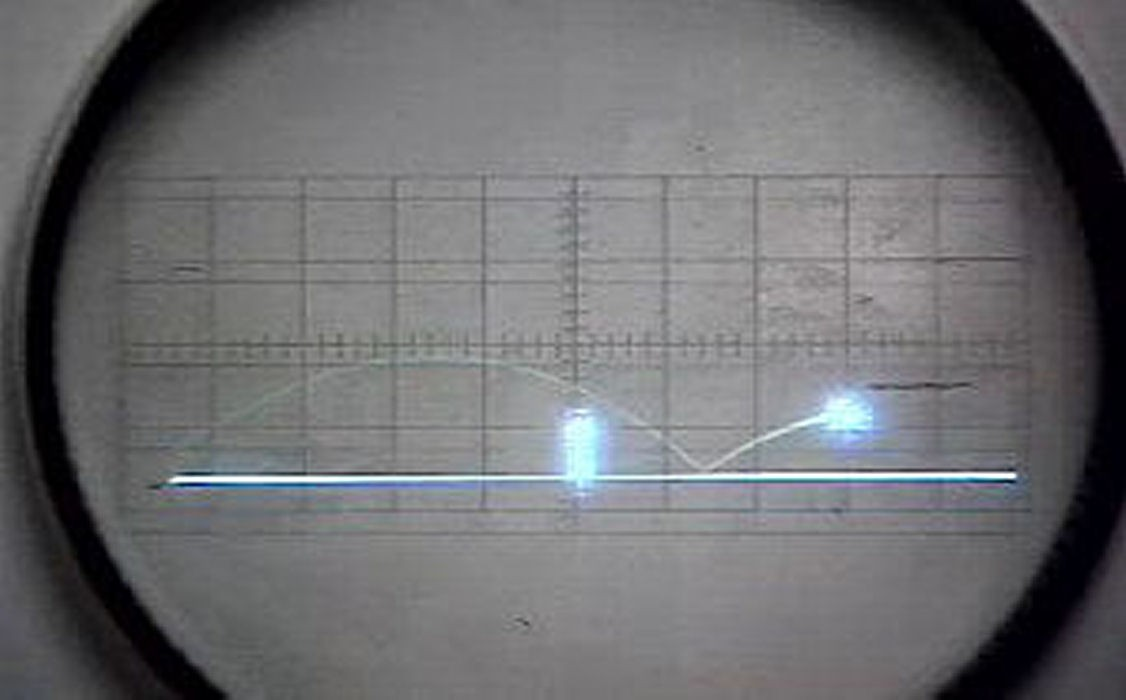
\includegraphics[width=0.7\textwidth]{img/tennis-for-two}
    \caption{Tennis For Two}
\end{figure}
Outros jogos surgiram nesta época, não muito mais complexos que o primeiro, mas sem grande evolução. Em 1958, um desses jogos se sobressaiu, primeiramente pelo número de patentes e depois pela interação incluir dois jogadores \textit{Tennis of Two}, desenvolvido pelo físico \textit{William Higinbotham}, sendo desenvolvido para entreter convidados no dia anual de visitas na \textit{Brookhaven National Laboratory}.\\
Em 1962, no \textit{MIT}, inspirado nas novelas de ficção científica de \textit{E. E. Smith}, \textit{Spacewar!}, assim como \textit{Tennis for Two} era jogado no osciloscópio e existiam várias variações do jogo espalhados pela universidade.\\
Mesmo com a queda dos preços dos componentes eletrônicos, no final dos anos sessenta e começo dos setenta, transformar \textit{Spacewar!} em um produto de entertenimento em casa era muito caro. Com o surgimento de uma nova geração de microcomputadores, como o \textit{DEC PDP-11}, o preço de computar caiu o suficiente para tornar possível jogos movidos a ficha, sendo pioneiros jogos como \textit{Sega Enterprises's Periscope (1967)} e \textit{Chicago Coin's Speedway (1968)}, que já incorporavam displays visuais e efeitos sonoros.\\
\begin{figure}[h!]
	\centering
    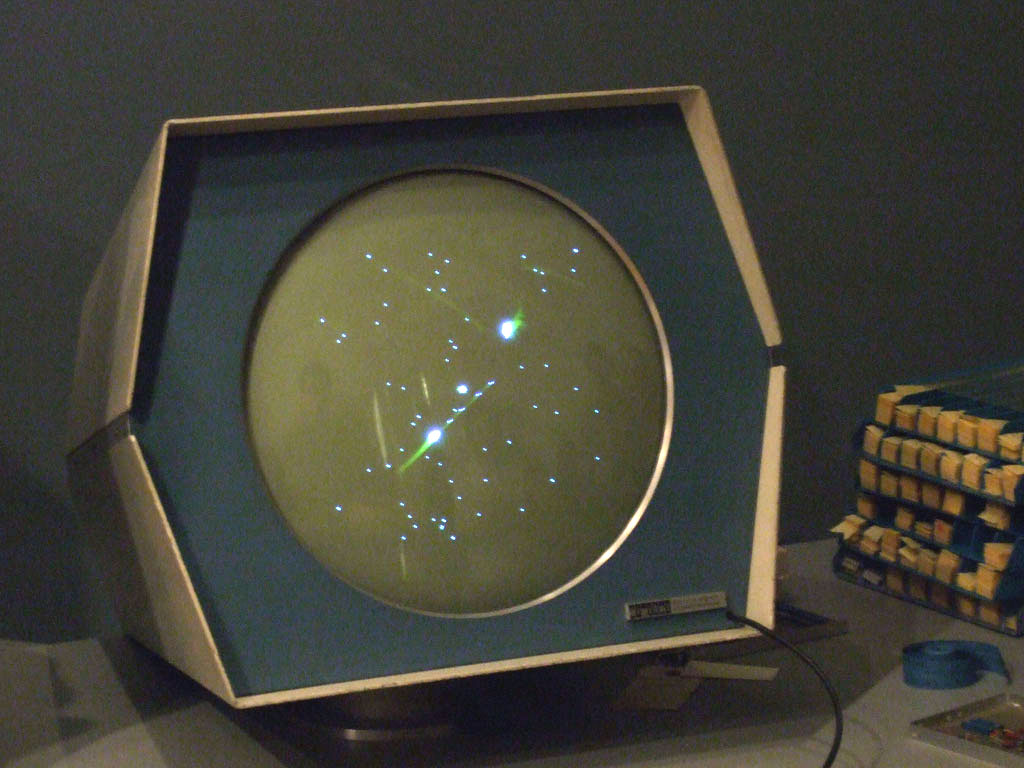
\includegraphics[width=0.7\textwidth]{img/spacewar}
    \caption{Spacewar!}
\end{figure}
\textit{Norlan Bushnell}, posteriormente fundador da Atari, em 1971 desenvolve um novo conceito de manipulação do tubo de raios catódicos de uma televisão cria uma nova versão do \textit{Spacewar!}, chamado \textit{Computer Space}, onde o jogador controla uma nave espacial e tem que destruir outros dois objetos voadores antes que eles o destruissem. Este jogo podia ser comprado e, devido ao custo e problemas de marketing, foi um fracasso.\\
Em 1966, \textit{Ralph Baer} e \textit{Bill Harrison}, criaram o primeiro video-game a ser jogado em uma televisão comum, chamado de \textit{Chase}.\\
Em 1969, um programador da AT\&T escreveu um jogo chamado \textit{Space Travel} para o \textit{Multics Operating System}, com o abandono da \textit{AT\&T} do projeto \textit{MULTICS} o jogo fora portado para o \textit{GECOS operating System} da \textit{GE}. Mais tarde o jogo foi considerado a primeira aplicação para \textit{UNIX}.\\
Em 1972, \textit{Bushnell} e \textit{Dabney} fundaram a \textit{Atari, Inc.} e lançaram Pong, o primeiro sucesso de jogos Arcade, vendendo 19.000 máquinas e criando muitas imitações.\\

\subsection{1ª Geração(1972-1977)}
\begin{figure}[h!]
	\centering
    \includegraphics[width=0.7\textwidth]{img/odyssey}
    \caption{Magnavox Odyssey}
\end{figure}
O primeiro consle caseiro, o \textit{Magnavox Odyssey}, foi desenvolvido por \textit{Ralph Baer} e associados, o desenvolvimento começou em 1966 com primeiro protótipo funcional em 1968 e lançamento em 1972. Usava cartuchos que eram basicamente constituídos de \textit{jumpers}, que habilitavam ou desabilitavam \textit{switchs}, alterando o circuito lógico. Propaganda intensa em televisão com o ator, diretor, produtor e cantor \textit{Frank Sinatra}, o Odyssey vendeu 100.00 cópias no primeiro ano e 2M enquanto fabricado. Pouco depois a Philips comprou a Magnavox e distribuiu o aparelho na Europa atingindo o sucesso de vendas.\\
\begin{figure}
	\centering
    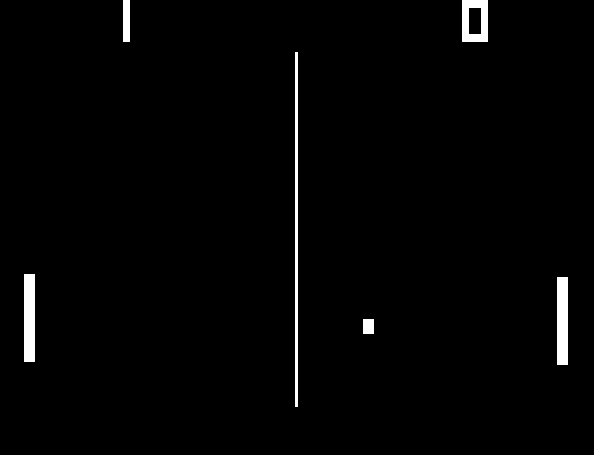
\includegraphics[width=0.7\textwidth]{img/pongpic}
    \caption{Jogo Pong}
\end{figure}
Em 1976, a \textit{Farchild Camera \& Instrument} lança seu \textit{Fairchild Channel F}, o primeiro videogame programável. Congelar o jogo, alterar o tempo e a velocidade passa a ser possível com \textit{Fairchild Channel F}. O \textit{joystick} era bem interessante: o botão ficava na ponta do manche e podia ser rotacionado. Assim, Pong ganhava inclinação na "raquete" e podia rebater a bolinha em vários ângulos.\\
\begin{figure}
	\centering
    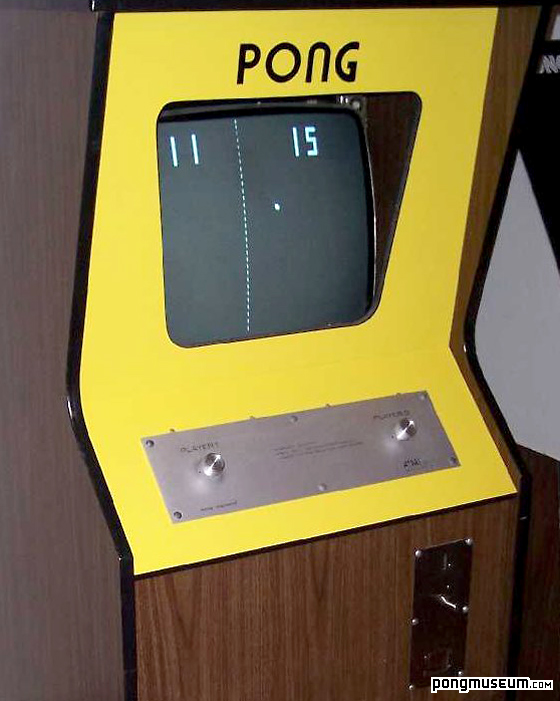
\includegraphics[width=0.4\textwidth]{img/pong2}
    \caption{Máquina Pong}
\end{figure}
Nessa época surgem as primeiras críticas a jogos violentos. \textit{Death Race}, da \textit{Exidy Games}, foi o precursor de \textit{Carmaggedon}. Sair atropelando tudo o que viesse pela frente era o objetivo do jogo. \textit{Death Race} serviu ainda de inspiração para a criação de outro jogo recente, \textit{Interstate 76}.\\
Com o mercado em crescimento, \textit{Bushnell} vende a \textit{Atari} para a \textit{Warner}, pois não vê outra maneira de mantê-la competitiva.\\

\subsubsection*{Crise dos Vídeo-Games de 1977}
Em 1977, fabricantes de velhos e obsoletos consoles e clones de \textit{Pong} vendem seus sistemas até a limpeza de estoque, criando um excesso no mercado e causando o abandono da \textit{Fairchild} e da \textit{RCA} de seus consoles. Apenas \textit{Atari} e \textit{Magnavox} permanecem no mercado de consoles caseiros por causa das perdas de 1977 e 1978.\\
A crise foi principalmente causada pelo número significante de clones de \textit{Pong} que transbordaram ambos o mercado de Arcade e consoles caseiros. A crise veio ao fim com o sucesso \textit{Space Invaders} da \textit{Taito} do Japão, em 1978, marcando a renascença da industria de jogos eletrônicos e pavilhando o caminho para a \textit{era de ouro dos jogos arcade}. Pouco depois sendo licensiado para o \textit{Atari VCS} (posteriormente conhecido como \textit{Atari 2600}), se tornando o primeiro grande hit e quadruplicando a venda de consoles caseiros.
\subsection{2ª Geração(1977-1983)}
\begin{figure}[h!]
	\centering
    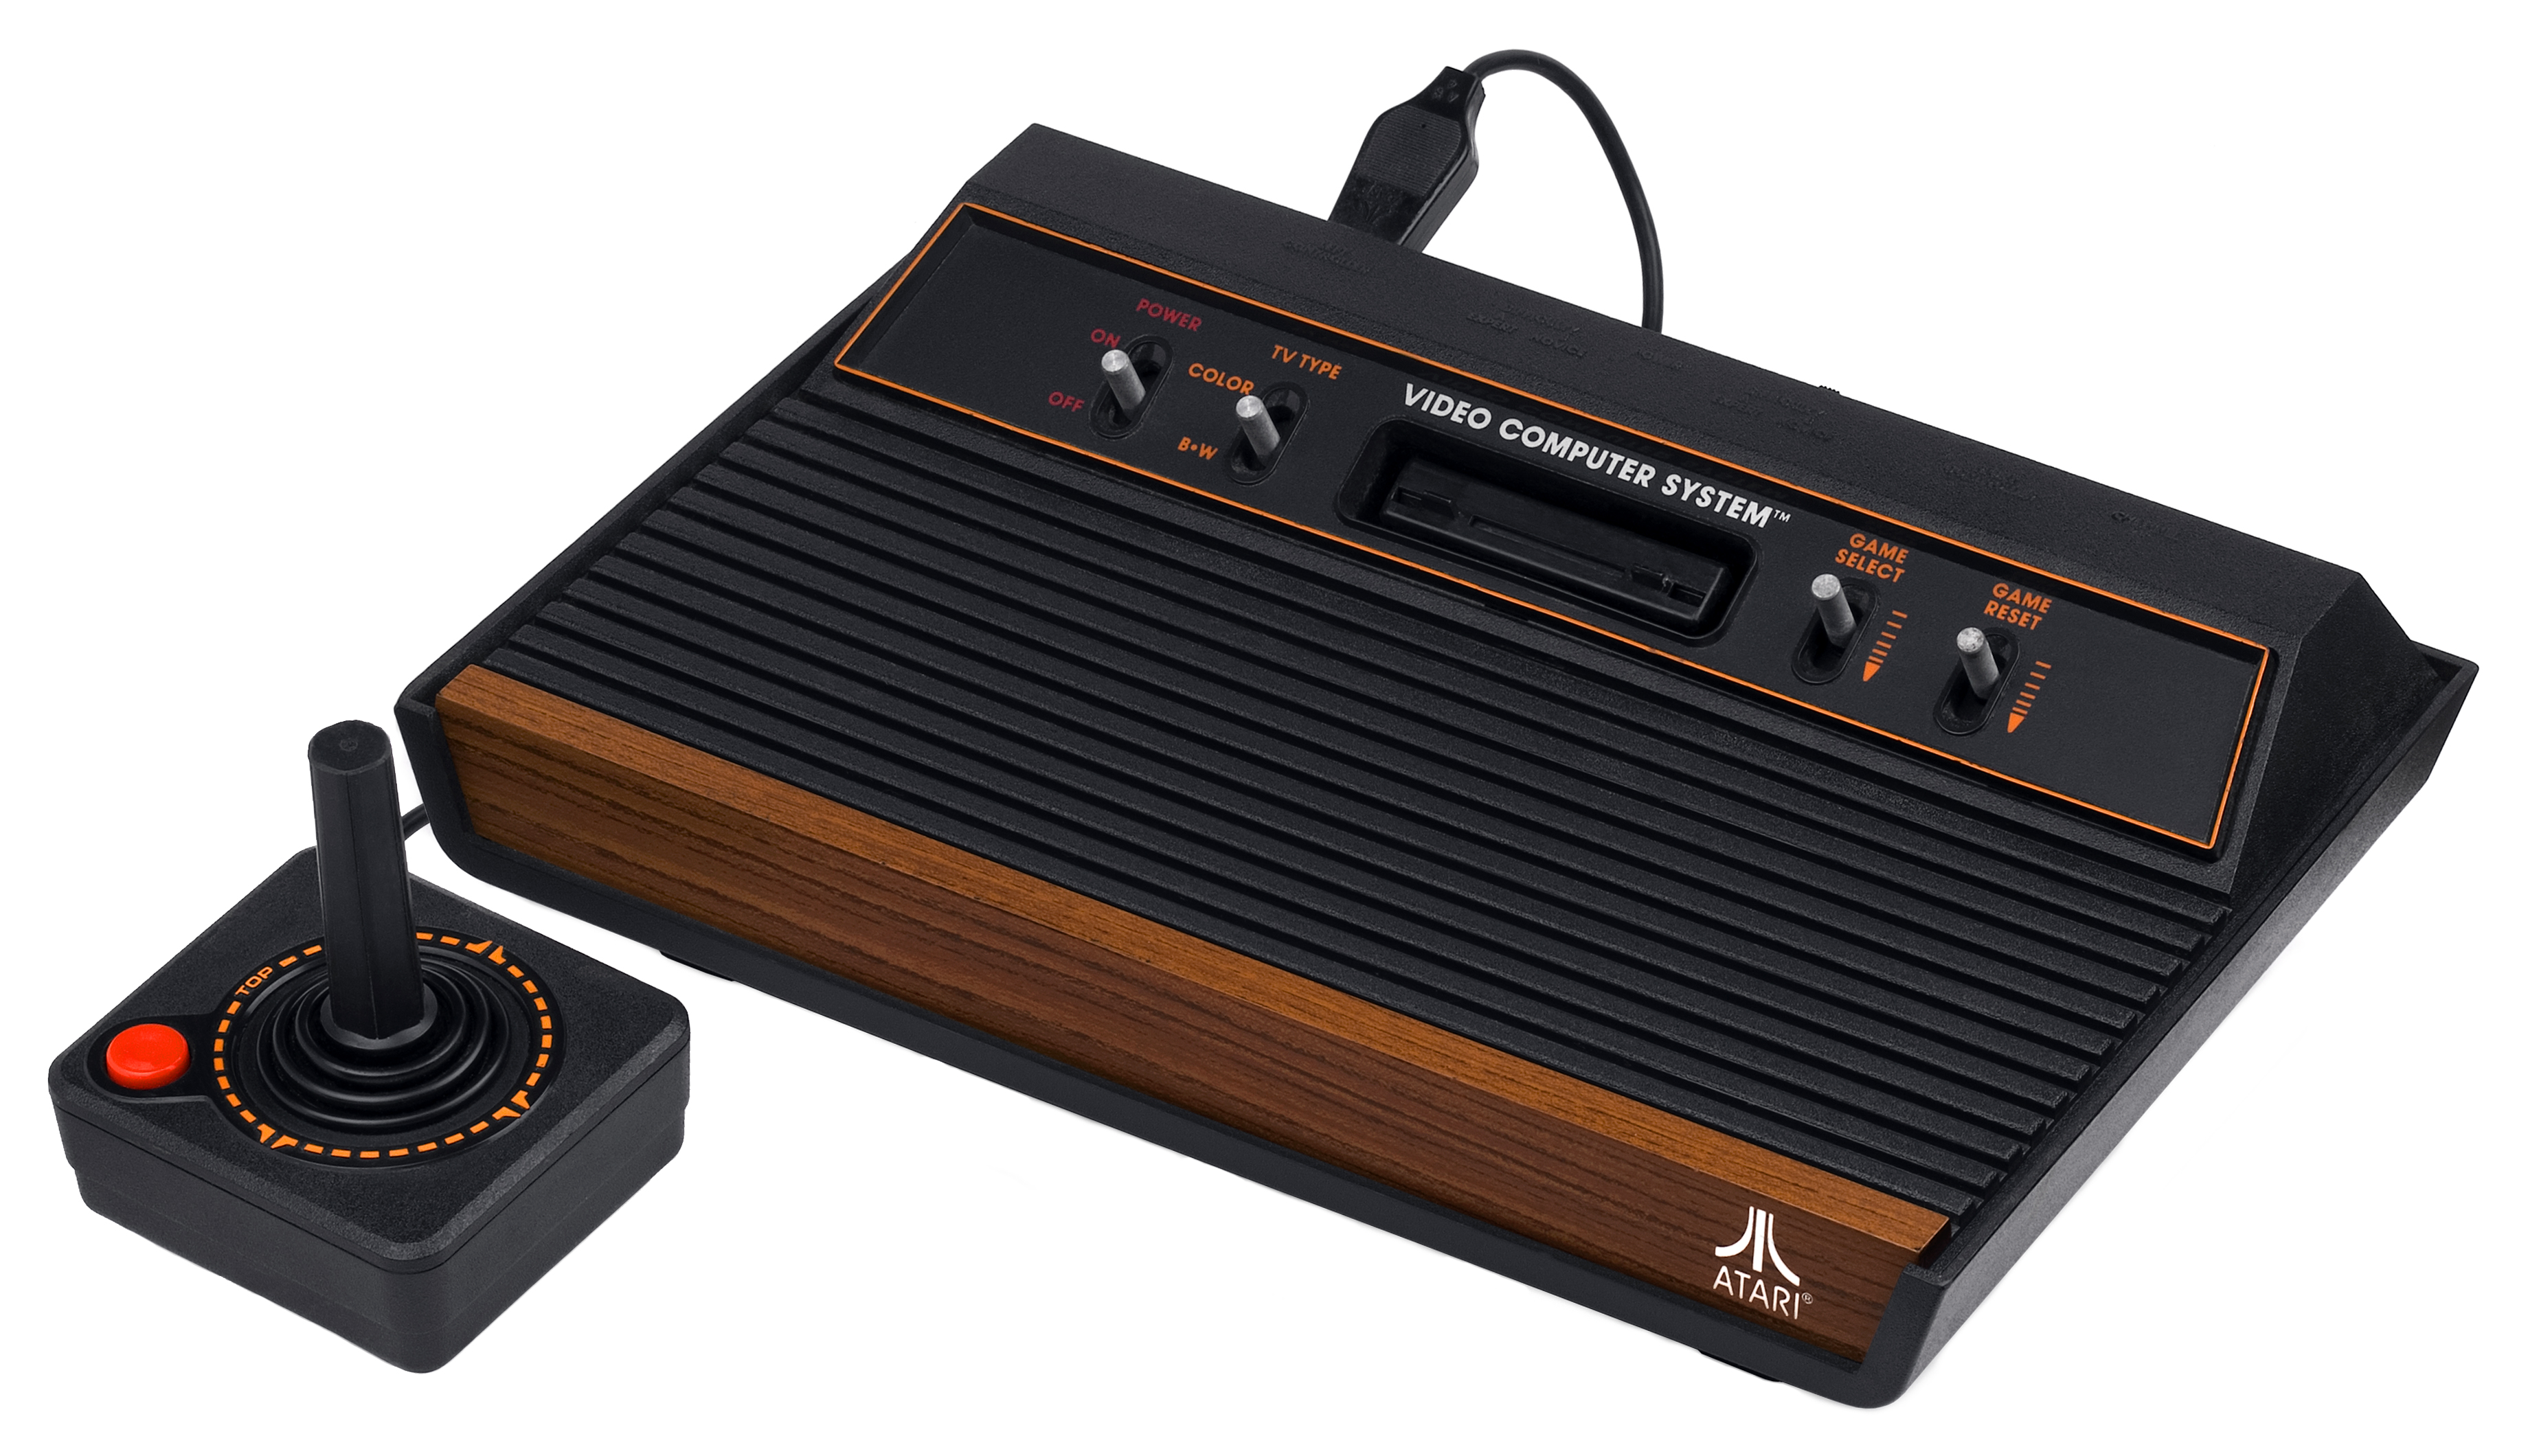
\includegraphics[width=0.4\textwidth]{img/atari}
    \caption{Atari 2600}
\end{figure}
Nos consoles anteriores, a lógica computacional para um ou mais jogos era implementada em microchips usando lógica discreta e nenhum jogo adicional poderia ser adicionado. Em outras palavras, estes consoles eram computadores de aplicação única, não programáveis. Isto obviamente era um problema para desenvolvedores, clientes tinham quem comprar comprar um novo device inteiro e acopla-los a tv para jogar jogos diferentes.\\
\begin{figure}[h!]
	\centering
    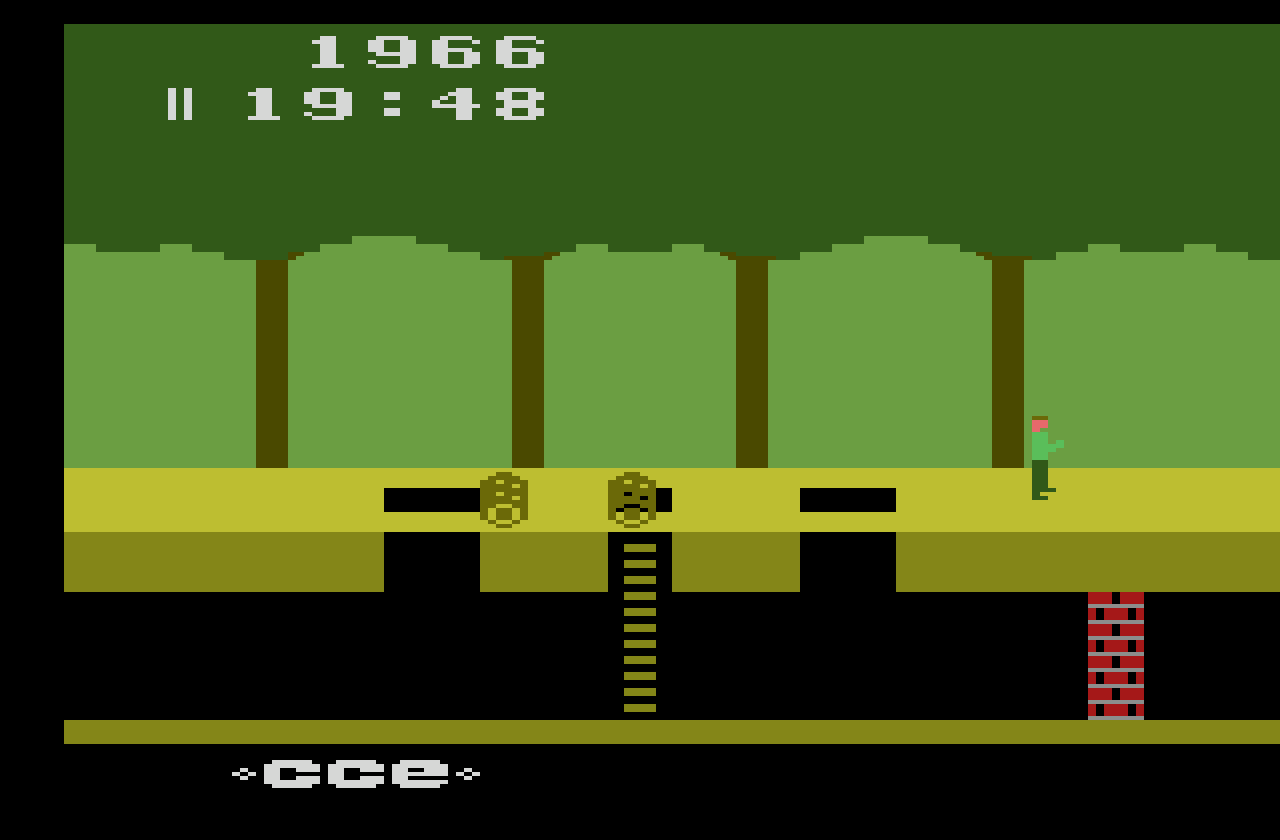
\includegraphics[width=0.7\textwidth]{img/pitfall}
    \caption{Pitfall para Atari 2600}
\end{figure}
Em meados dos anos 70, jogos continham microprocessadores de propósito geral e jogos eram encontrados em cartuchos, começando em 1976, com o lançamento do \textit{Fairchild Video Entertainment System (VES)}. Programas eram gravados em chips ROM(ICs) que eram montados em cartuchos de plástico que podiam ser plugados nos consoles. Quando o cartuchos era plugado, a ROM eletricamente se tornava parte do microcomputador do console, consumidores podiam agora ter bibliotecas de jogos. Entretanto, produção de video-games ainda era habilidade de nichos específicos. Warren Robinett, um famoso programador do jogo Adventure, cita: "In those old far-off days, each game for the 2600 was done entirely by one person, the programmer, who conceived the game concept, wrote the program, did the graphics—drawn first on graph paper and converted by hand to hexadecimal—and did the sounds".\\
Três máquinas dominaram essa geração nos EUA, de longe superando outros rivais:\\
\begin{itemize}
\item O \textit{Video Computer System (VCS)}, console baseado em cartuchos, posteriormente chamado de \textit{Atari 2600}, foi lançado em 1977 pela Atari(1983 no Brasil). Nove jogos foram lançados junto com ele para a temporada de férias. Enquanto teve um inicio lento, a adaptação do jogo \textit{Space Invaders} se tornou o "\textit{jogo matador}" e quadruplicou as vendas do console. Pouco depois o \textit{Atari 2600} se tornou rapidamente o mais popular de todos os video-games da geração até a crise de 1983. Notavelmente o VCS vinha apenas com uma CPU 8-bit 6507, 128 bytes (i.e. 0.125 KB) de RAM, e no máximo 4 KB de ROM em cada cartucho.\\
\item O \textit{Intellivision}, introduziu o Mattel em 1980. Apesar de cronologicamente pertencer a \textit{geração 8-bit}, o \textit{Intellivision} tinha um único processador com instruções que eram de 10 bits de largura(aceitando mais instruções maior potencial de velocidade), e registradores de 16 bits de largura. O sistema, que possuia gráficos superiores ao do velho Atari 2600, foi inferior em popularidade, mas ainda assim um sucesso.\\
\item O \textit{ColecoVision}, uma máquina ainda mais poderosa, apareceu em 1982. Com uma adaptação do jogo de arcade \textit{Donkey Kong} incluso no pacote, também decolou em vendas. \\
\end{itemize}
Entretanto, a presença de 3 consoles principais no mercado e o excesso de jogos de qualidade baixa no mercado sobrecarregou o as prateleiras e eradicou consumidores no interesse por jogos. Em um ano este mercado entrou em crise.
Em 1979, \textit{Activision} foi fundado por ex-programadores da Atari "que perceberam que os jogos tinham sido desenvolvidos anonimamente nos seus salários de U\$20.000 eram responsáveis por 60 porcento dos U\$100 milhões de lucros anuais da empresa". Este foi o primeiro desenvolvedor de jogos independente. Em 1982, aproximadamente 8 milões de casas americanas possuiam consoles, e as vendas de consoles caseiros chegaram a U\$3.8 bilões, que era aproximadamente metade dos U\$8 bilhões das vendas de jogos arcade.\\
No inicio dos anos 80 também começam a ficar populares jogos para computadores PC.\\
\subsubsection*{Crise dos Vídeo-Games de 1983}
No final de 1983 a indústria de jogos sofreu perdas ainda maiores que na crise de 1977, também a falência de diversas empresas de computadores pessoais e consoles de vídeo-games. As causas incluem a produção de jogos pouco desenvolvidos, uma imatura distribuição de sistema que fez com que revendedores tivessem seus estoques cheios mesmo com descontos. Além de um pensamento geral dos revendedores que os computadores pessoais seriam a próxima grande coisa em termos de entertenimento.

\subsection{3ª Geração(1983-1995)(8-bit)}
\begin{figure}[h!]
	\centering
    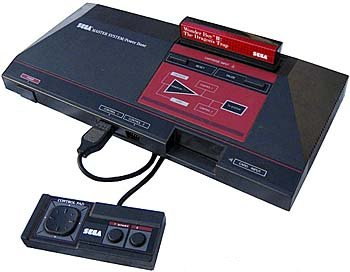
\includegraphics[width=0.4\textwidth]{img/mastersystem}
    \caption{Master System}
\end{figure}
Em 1985 o mercado americano de vídeo-games foi revivido com o lançamento do console 8-bit da Nintendo, Famicom na Ásia, NES nos EUA. Seu lançamento original oferecia 3 pacotes diferentes, um sem jogo e dois controles, outro com o \textit{Super Mario Bros} e dois controles e outro com R.O.B., um light zapper, 2 gamepads, e dois game packs: Gyromite, and Duck Hunt. Outros pacotes foram oferecidos posteriormente. O NES se tornou sucesso instantaneo no mercado japonês e americano de jogos, dominando ambos os mercados até a geração seguinte.\\
\begin{figure}[h!]
	\centering
    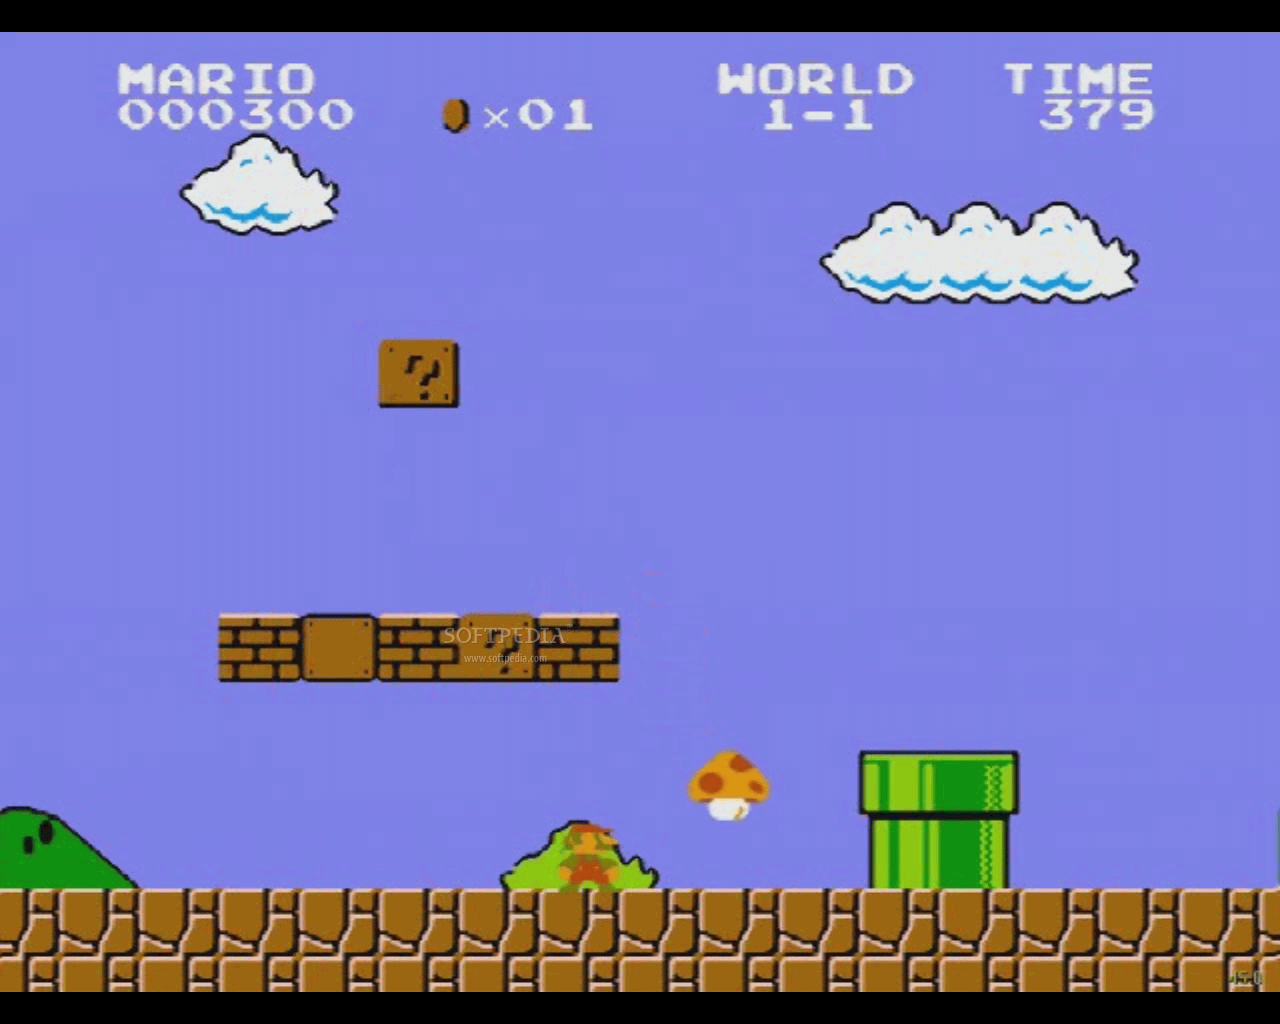
\includegraphics[width=0.8\textwidth]{img/mario}
    \caption{Super Mario Bros para NES}
\end{figure}
Outros mercados não foram dominados fortemente pela nintendo pela força dos computadores pessoais, abrindo espaço para outros consoles como Master System na Austrália e no Brasil.\\
Também nesta geração o gamepad se tornou o principal controle em relação aos outros tipos, como joysticks, paddles e keypads.\\
O fim da geração se deu com a dicontinuação do nintendo 8-bit.\\
\subsection{4ª Geração(1987-1999)(16-bit)}
\begin{figure}[h!]
	\centering
    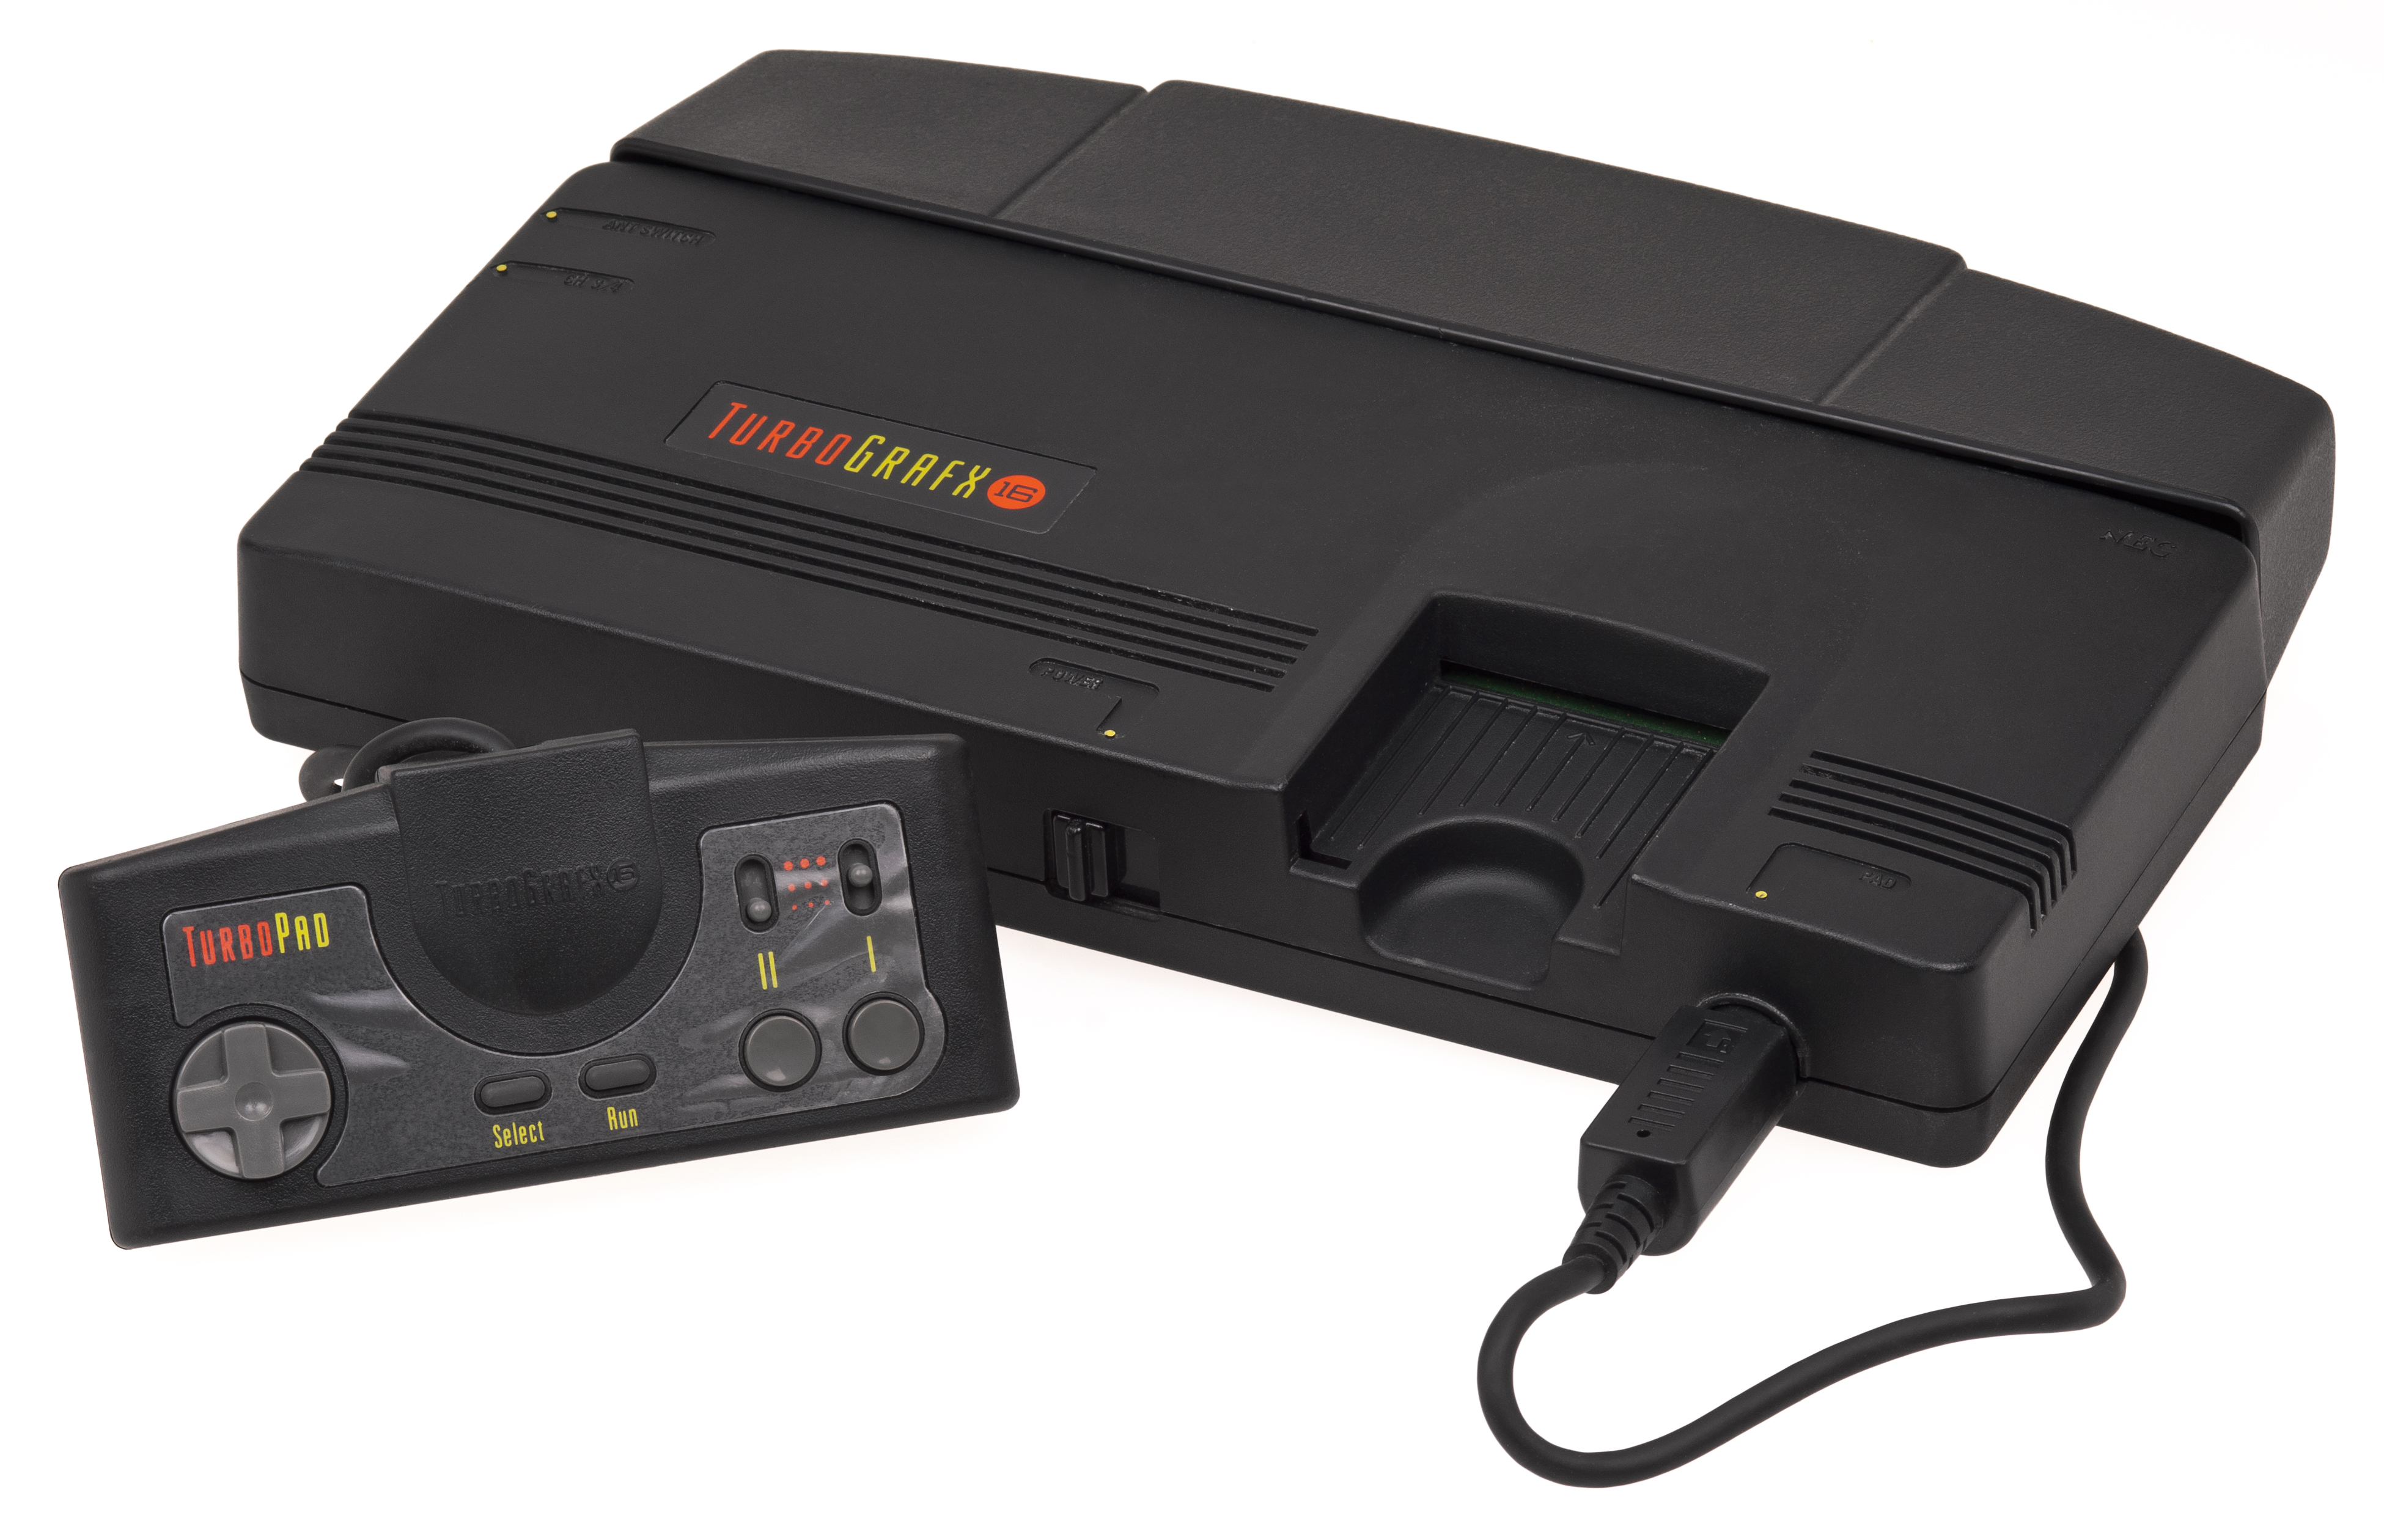
\includegraphics[width=0.6\textwidth]{img/turbografx}
    \caption{TurboGrafx-16}
\end{figure}
Esta geração começou com o lançamento do \textit{Sega Master System/Genesis} em 1988 que entra no mercado para concorrer com a Nintendo. Esta responde em 1990 com seu \textit{Super NES(SNES)}. Apesar de ser marcado como o primeiro 16-bit o \textit{TurboGrafx-16}, lançado em 1987, ela possuia processador central de 8-bit, apenas o processador gráfico deste era 16-bit.\\
\begin{figure}[h!]
	\centering
    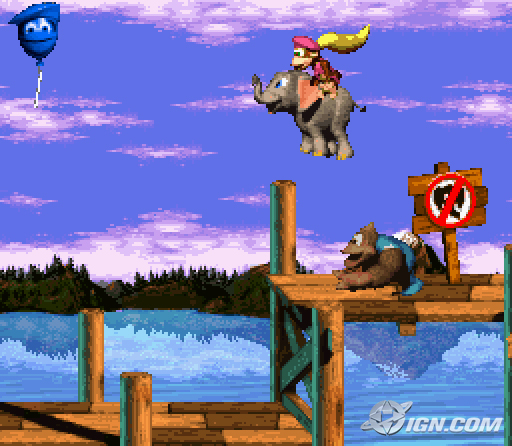
\includegraphics[width=0.7\textwidth]{img/dk3}
    \caption{Donkey Kong Country 3 para SNES}
\end{figure}
No Japão, o \textit{PC Engine}, como era conhecido o \textit{TurboGrafx-16} lá, teve sucesso sobre o \textit{NES}, e o drive de CD permitiu afastar a entrada do \textit{Mega Drive/Genesis}. \\
Drives de CD foram vistos pela primeira vez nesta geração, no \textit{PC Engine} em 1988, como um periférico, e no \textit{Mega Drive} em 1991.\\
Gráficos básicos em 3D ficaram populares com poligonos projetados habilitados a partir de processadores adicionais dentro dos cartuchos como \textit{Virtua Racing} e \textit{Star Fox}, e ocasionalmente sem processadores especiais, assim como modelos poligonais da adaptação para \textit{Genesis} de \textit{Hard Drivin'}, que tinha gráficos poligonais 3D purosno processador  ~8 MHz 68000 usando modelos poligonais extremamente simplificados, a um \textit{frame rate} menos que 4 fps, e baixa resolução.\\
\textit{SNK's Neo-Geo} era o console mais caro com uma margem grande de diferença quando fora lançado em 1990, e permaneceu assim por anos. Este também era capaz de gráficos 2D em qualidade anos a frente de seus concorrentes. A razão disto foi que o hardware encontrado nos consoles era o mesmo que os das máquinas arcade da empresa na época. Esta tinha sido a primeira vez, desde as máquinas de \textit{Pong} caseiras que um console trazia a experiência real de um arcade para ambiente domiciliar.\\
Esta geração terminou com a discontinuação do \textit{SNES}, em 1999.
\subsection{5ª Geração(1993-2006)(32 e 64-bit)}
Em 1993, a \textit{Atari} entra novamente no mercado de jogos com o \textit{Atari Jaguar}. Também em 1993, \textit{The 3DO Company} lança seu \textit{3DO Interactive Multiplayer}, que foi amplamente divulgado e promovido, mas falhou frente ao \textit{Jaguar} pelo alto preço. Ambos os consoles com vendas baixas e jogos de pouca qualidade. \\
\begin{figure}[h!]
	\centering
    \includegraphics[width=0.7\textwidth]{img/n64}
    \caption{Nintendo 64}
\end{figure}
Em 1994, no Japão, 3 video-games foram lançados: o \textit{Sega Saturn}, o \textit{Sony Playstation} e o \textit{PC-FX}, os dois primeiros sendo lançados também nos EUA em 1994. O \textit{Playstation} rapidamente passou os concorrentes em termos de qualidade dos titulos, com excessão do velho \textit{SNES}, que ainda tinha suporte da maioria das desenvolvedoras de jogos. \\
Em 1995 a Nintendo lançou o Virtual Boy, com baixas vendas devido ao pouco suporte de terceirizadas e a tela monocromática. Em 1996 o Virtual Boy foi descontinuado.\\
\begin{figure}[h!]
	\centering
    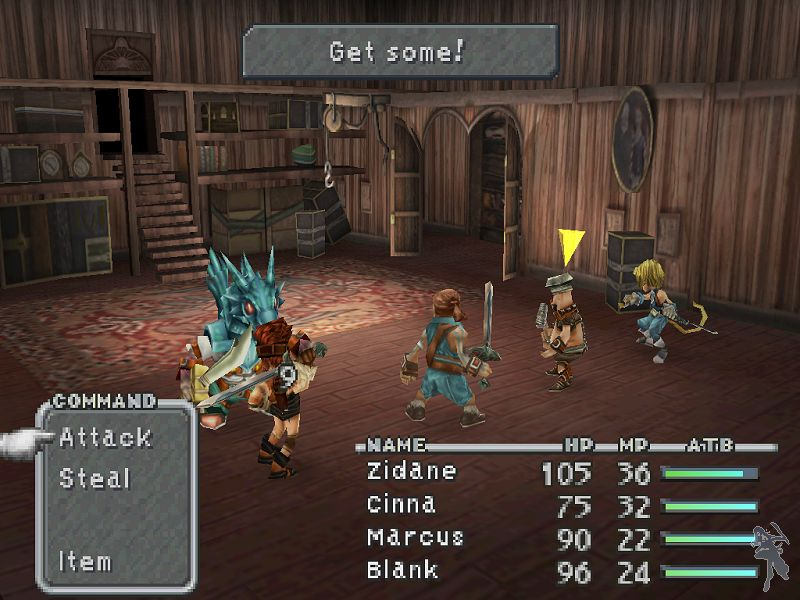
\includegraphics[width=0.7\textwidth]{img/ff9}
    \caption{Final Fantasy IX para Playstation}
\end{figure}
Depois de muitos atrasos, durante o qual o \textit{Sony Playstation} ganhou aceitação da industria, a Nintendo lança seu console 64-bit, o Nintendo 64, em 1996. Novamente a Nintendo optou por usar cartuchos ao invés de CDs, o único da geração, o que tinha como vantagens a velocidade de acesso as informações e a segurança contra pirataria, e mostrou-se desvantajoso devido a baixa capacidade(64MB, contra 690MB dos CDs) e o maior custo de fabricação, levando companhias que antes produziam exclusivamente para a Nintendo para outras plataformas, como a \textit{Square Enix}, que criou a série \textit{Final Fantasy}.\\
Até o fim do periodo a Sony tornou-se a lider do mercado. A geração termina com a discontinuação do \textit{Playstation}.
\subsection{6ª Geração(1998-2013)}
Esta geração é marcada pelo fim da \textit{Sega} no mercado de hardware, a queda da \textit{Nintendo}, a solidificação da \textit{Sony} e a entrada da \textit{Microsoft} como produtora de consoles.\\
\begin{figure}[h!]
	\centering
    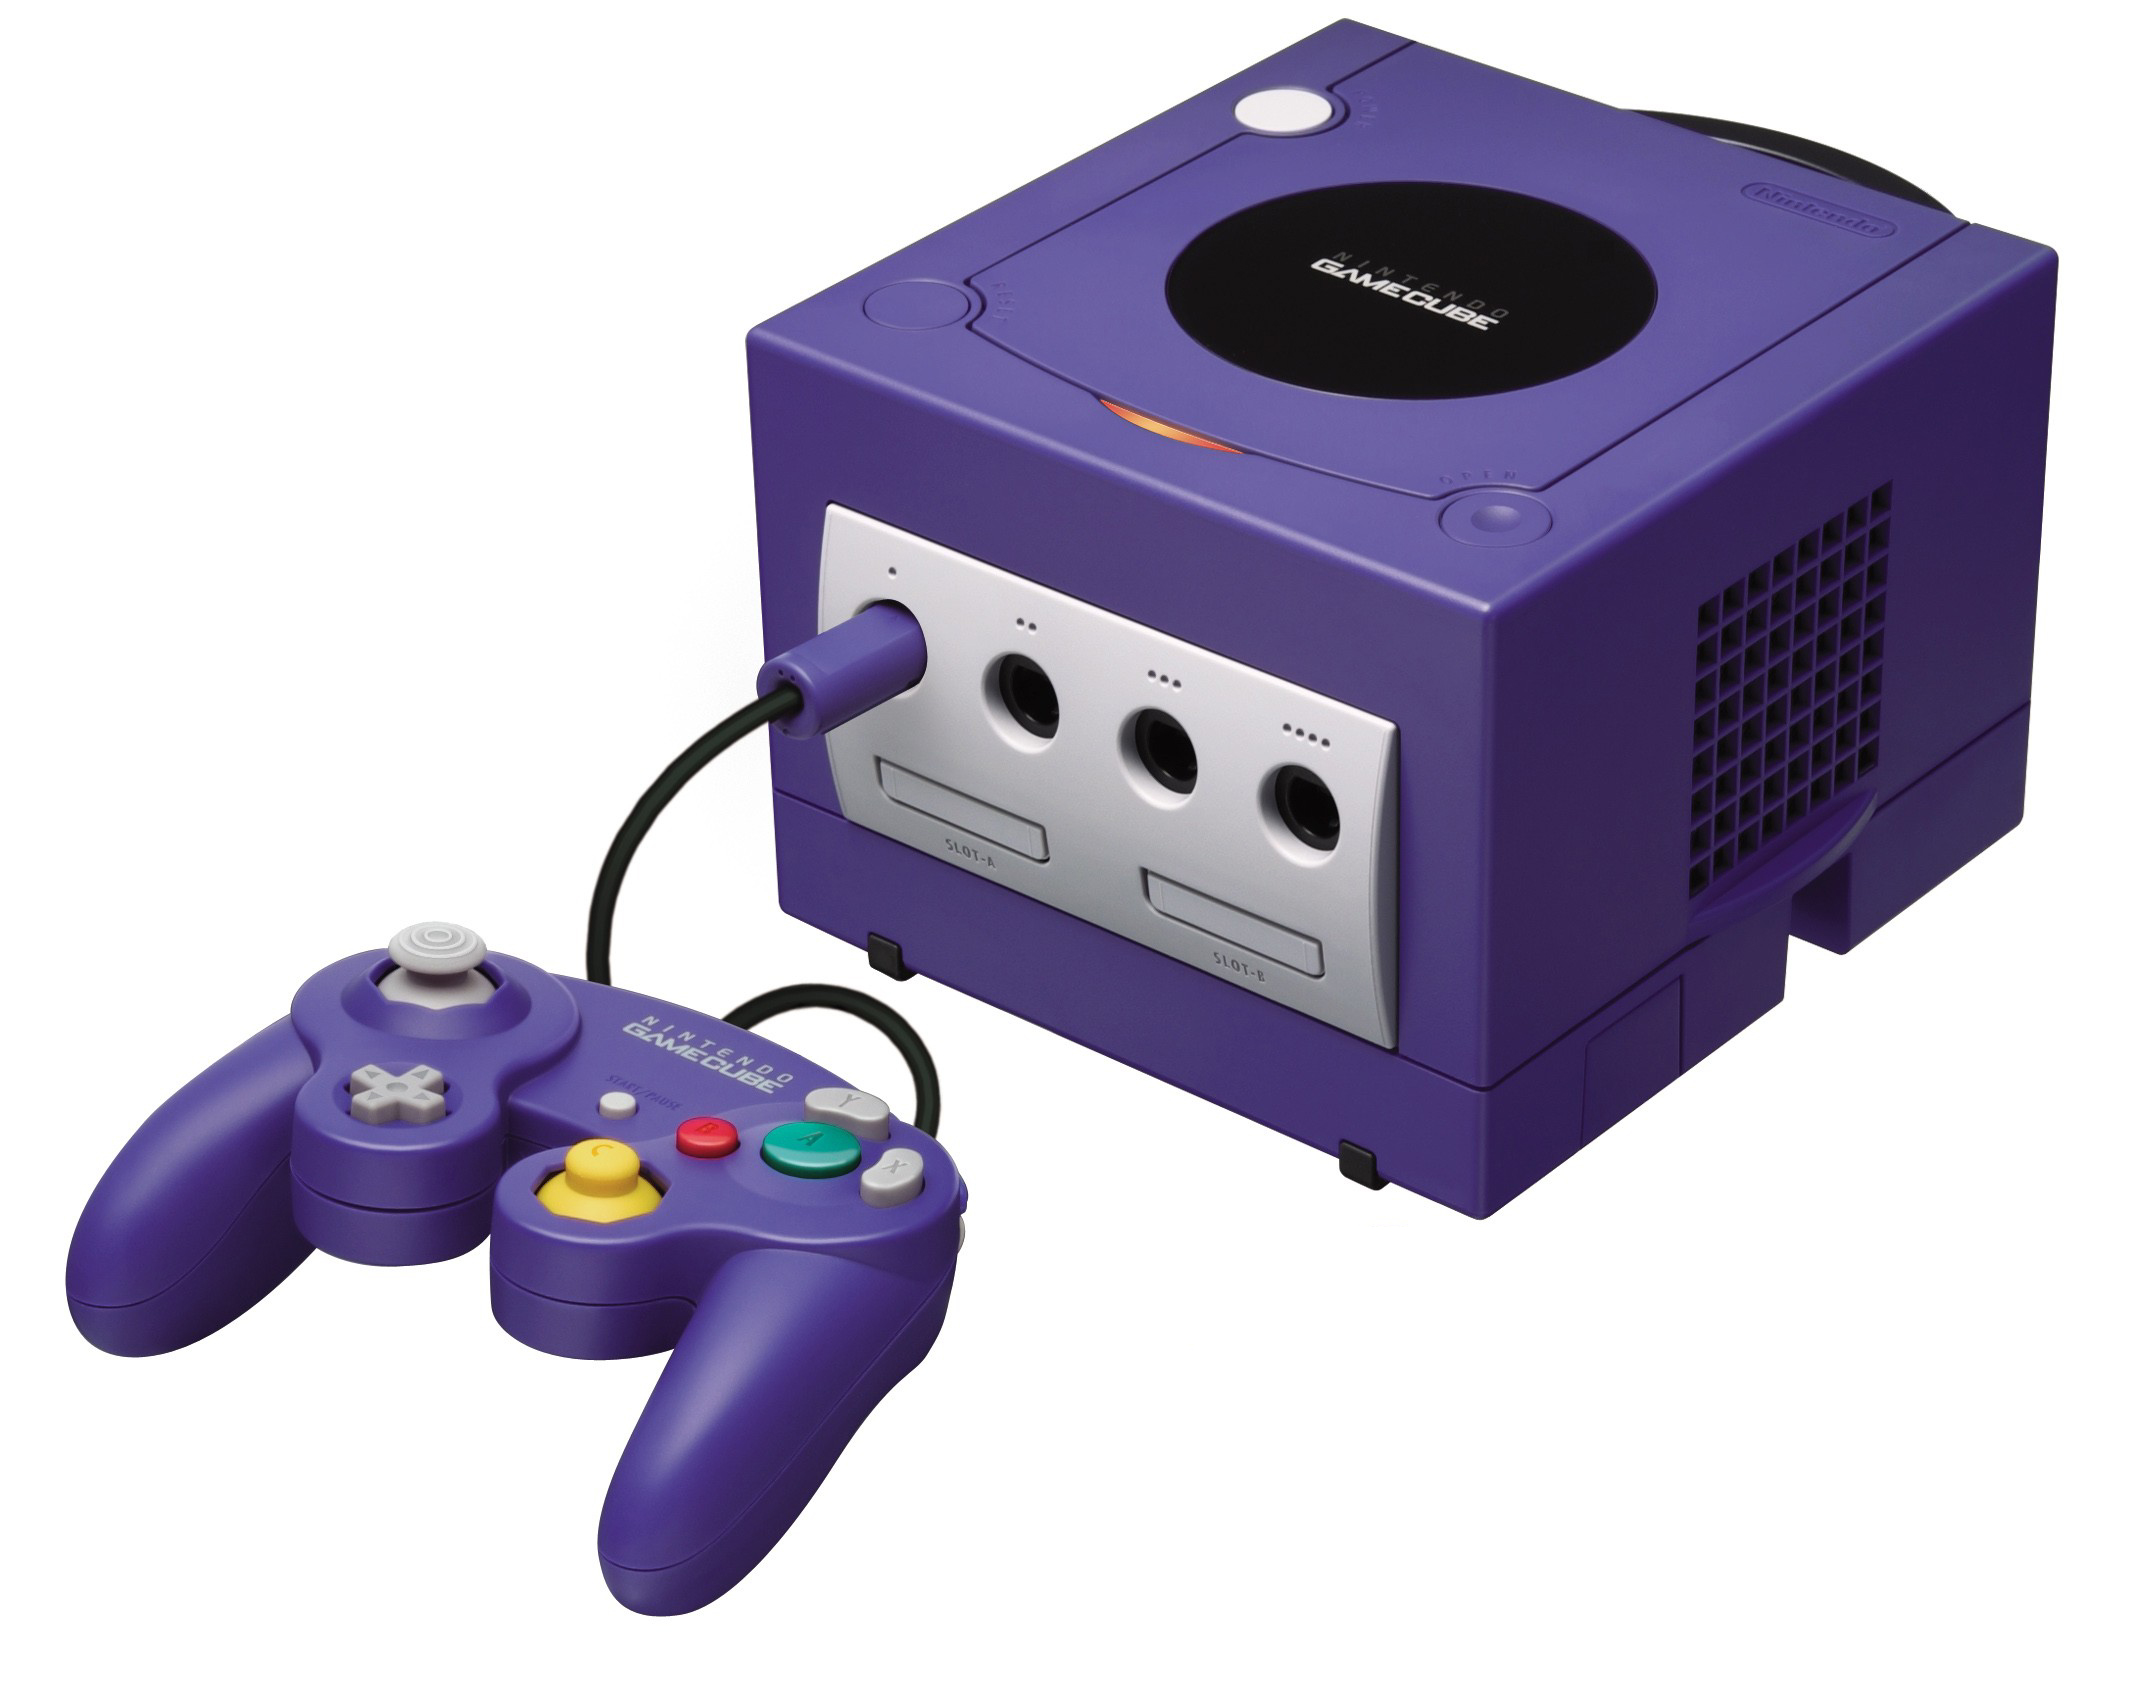
\includegraphics[width=0.7\textwidth]{img/gamecube}
    \caption{Nintendo Game Cube}
\end{figure}
Esta geração foi aberta com o \textit{Dreamcast} em 1998. Este foi o primeiro console com suporte a internet e jogo online. Apesar do sucesso inicial logo decaiu ao ponto de a Sega dedicar-se apenas aos jogos nas gerações seguintes.\\
O segundo da geração foi o \textit{Playstation 2}, que usava discos de DVD com capacidades de processamento e gráficos muitos superiores aos antecessores.\\
\begin{figure}[h!]
	\centering
    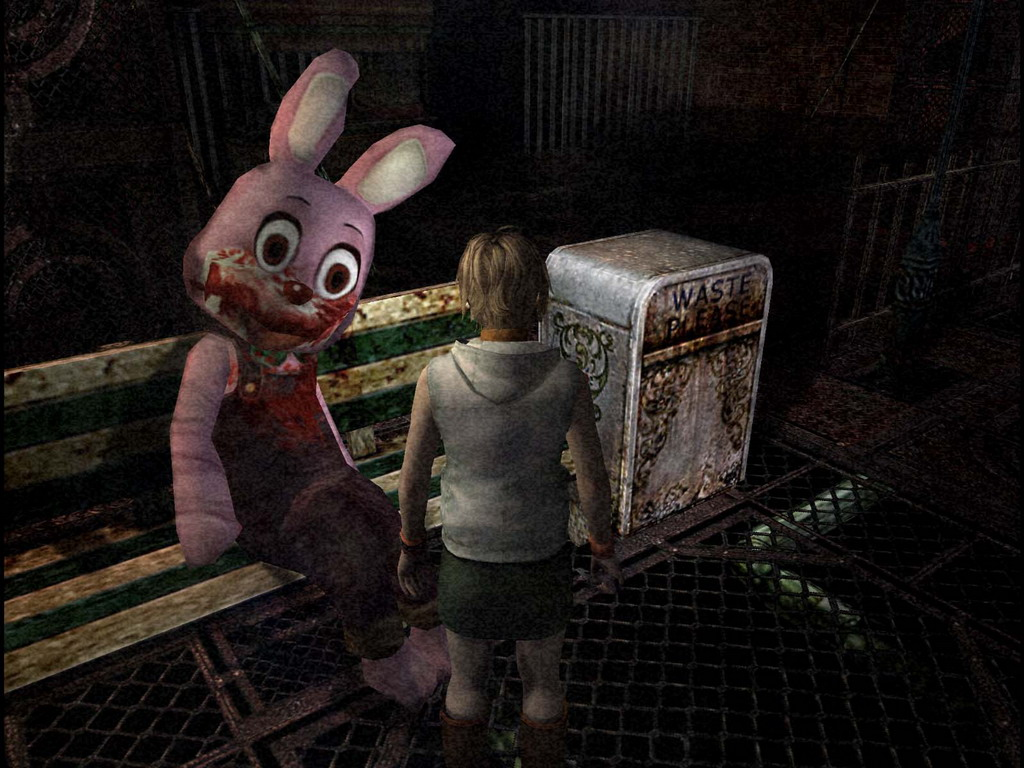
\includegraphics[width=0.7\textwidth]{img/sh3}
    \caption{Silent Hill 3 para Playstation 2}
\end{figure}
Um ano depois a \textit{Nintendo} lança o \textit{Game Cube}, que usava discos \textit{mini-DVD} de 1.4GB, 200 vezes mais que no \textit{Nintendo 64}. Devidos as capacidades do Playstation 2 e da antecipação do console a \textit{Nintendo} perdeu ainda mais espaço, sobrando apenas alguns poucos desenvolvedores exclusivos. Para piorar o console ganhou a reputação de vídeo-game para crianças.\\\\
Antes do fim de 2001, a \textit{Microsoft} lançou seu \textit{XBOX}, que tinha como principais características a facilidade de converter jogos PC em jogos XBOX, e teve sucesso instantâneo devido ao lançamento do jogo \textit{Halo: Combat Evolved}. Até o fim da geração o \textit{XBOX} havia superado as vendas do \textit{Game Cube}.\\
Em 2001 a Nintendo lança seu portátil Game Boy Advanced, o que manteve a Nintendo no mercado de consoles, tendo neste nicho apenas o fracasso N-Gage da Nokia.\\
Nesta geração vieram os primeiros protótipos de controles da geração seguinte.
A geração acabou com a descontinuação do \textit{Playstation 2} pela \textit{Sony} em 2013.

\subsection{7ª Geração(2004-Presente)}
\begin{figure}[h!]
	\centering
    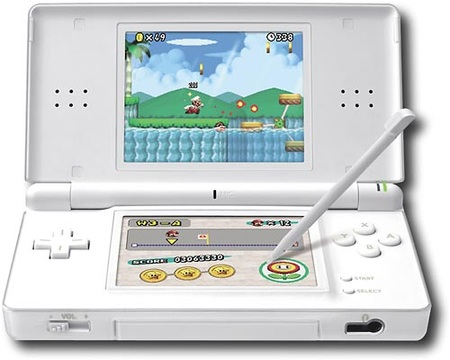
\includegraphics[width=0.7\textwidth]{img/nds}
    \caption{Nintendo DS}
\end{figure}
A geração começa primeiramente com o lançamento dos portáteis \textit{Nintendo DS} e \textit{Sony Playstation Portable(PSP)} em 2004. Eles tinham capacidades diferentes, a Sony apostou em melhores gráficos 3D e processamento e a Nintendo em jogabilidade com duas telas sendo uma dela sensível ao toque.\\
\begin{figure}[h!]
	\centering
    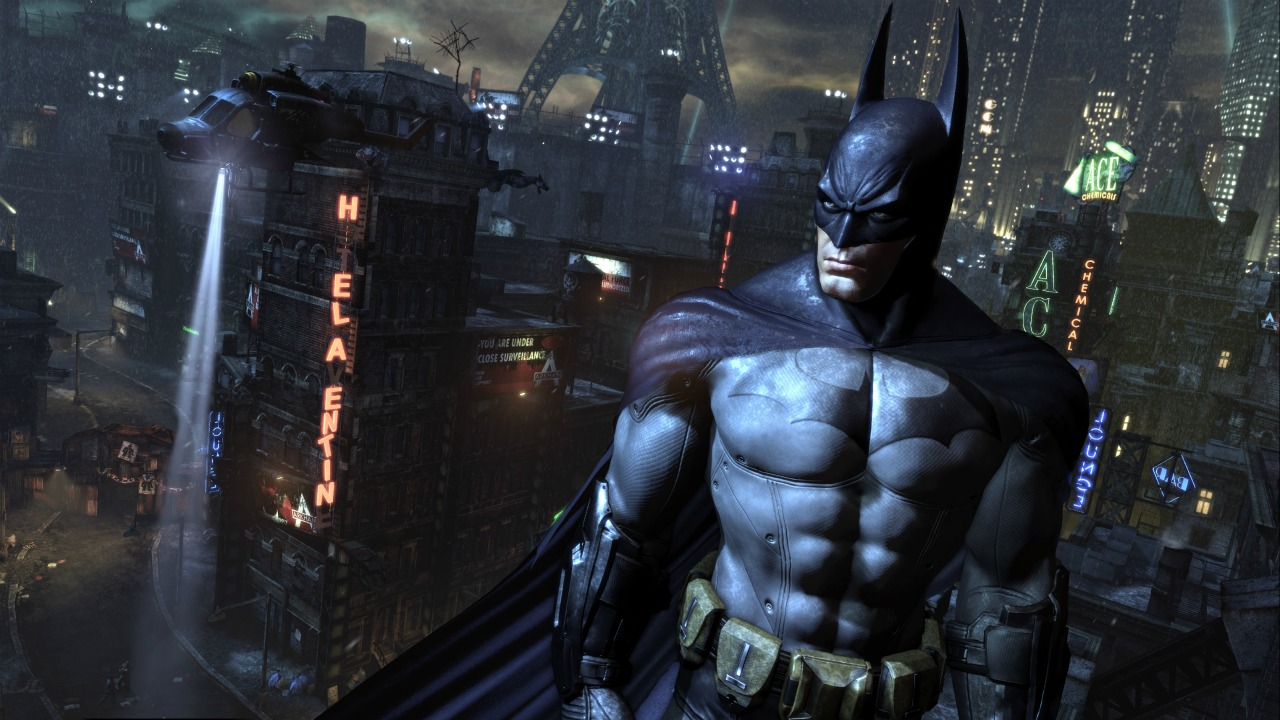
\includegraphics[width=0.7\textwidth]{img/bac}
    \caption{Batman Arkham City para Xbox360 e Playstation 3}
\end{figure}
Em consoles a Microsoft lança primeiro com seu \textit{XBOX360} em 2005, a Sony segue em 2006 com o \textit{Playstation 3(PS3)}. Ambos os consoles com alta definição de imagem através de porta HDMI, armazenamento em disco, jogo e venda online e \textit{wi-fi}. O PS3 vem com leitor blu-ray enquanto o XBOX360 com leitor de DVD, como na geração anterior.\\
\begin{figure}[h!]
	\centering
    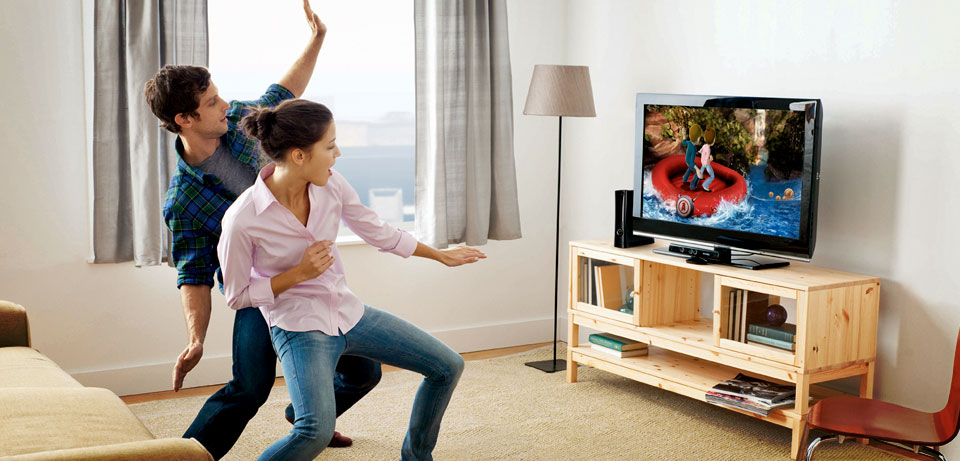
\includegraphics[width=0.7\textwidth]{img/kinect}
    \caption{Kinect para XBOX 360}
\end{figure}
Pouco depois do lançamento do PS3, ainda em 2006, a \textit{Nintendo} lança seu \textit{Wii}, com modesto avanço em hardware comparado com o \textit{Game Cube}. Conseguiu sucesso devido ao seu inovador controle com sensor de movimento e pelo seu baixo custo comparado aos concorrentes. Seu controle permitia a criação de controles alternativos, como raquetes, espadas, escudos, armas de fogo, tacos de baseball e outros. Com o sucesso do console a \textit{Nintendo} dominou o mercado de jogos casuais.\\
Devido ao sucesso do controle do \textit{Wii} a \textit{Sony} lança sua camera \textit{Playstation eye} e seu controle "\textit{wii-like}" \textit{Playstation Move} em 2010, que vendeu 8.8 milhões de cópias em menos de 1 ano.\\
Também em 2010 a \textit{Microsoft} lança seu \textit{Kinect} para XBOX360, onde o controle passa a ser o corpo do proprio jogador, vendendo 8 milhões de cópias em 60 dias.
\subsection{8ª Geração(2011-presente)}
\begin{figure}[h!]
	\centering
    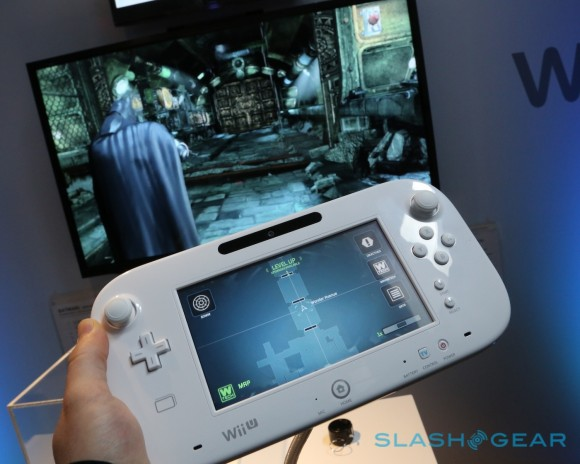
\includegraphics[width=0.7\textwidth]{img/wiiu}
    \caption{Nintendo Wii U}
\end{figure}
No final de 2011 a Sony lança seu novo portátil, o Playstation Vita. Com alta-definição, possibilidade de 3G.\\
\begin{figure}[h!]
	\centering
    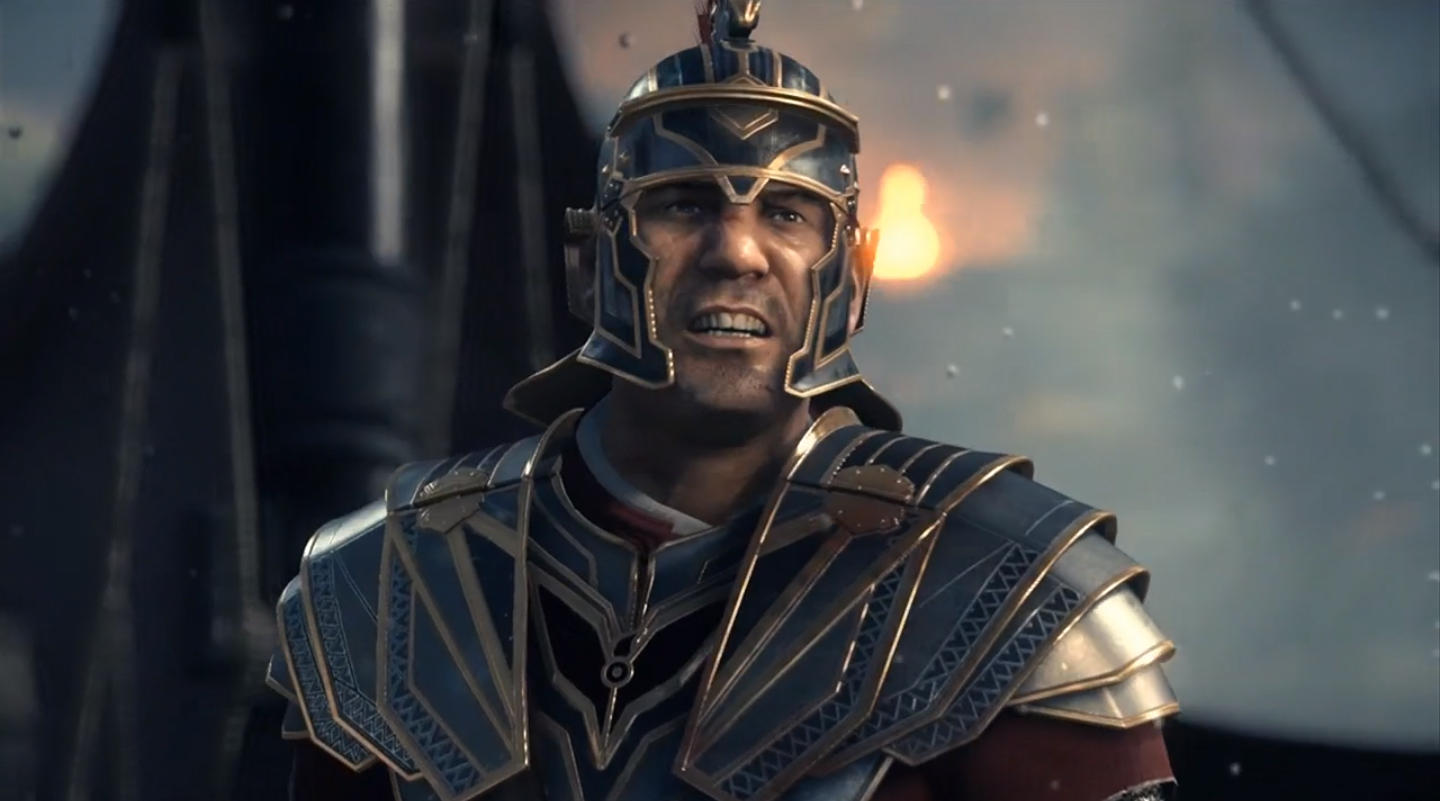
\includegraphics[width=0.7\textwidth]{img/ryse}
    \caption{Ryse para XBox One}
\end{figure}
Em 2012, a Nintendo lança o sucessor do \textit{Wii}, o \textit{Wii U}, que começa oficialmente a 8ª geração, suportando alta-defnição de imagem, tela adicional no controle do jogador, provendo informação adicional e gameplay assíncrono.\\
No final de 2013, o lançamento do \textit{Playstation 4(PS4)} e do \textit{XBOX One(XONE)} marcam a entrada das outras duas companhias principais de consoles.\\
Esta geração também é marcada pela futura promessa de entrada de outras companhias no mercado, como a \textit{Valve}, com sua \textit{Steam Machine}, carregando o nome do popular distribuidor de jogos, \textit{Steam}, entre gamers de PC, Mac e Linux.


\section{O SNES}
O Super Nintendo Entertainment System é um vídeo-game de 16 bits desenvolvido pela Nintendo e lançado em 1990 no Japão, 1991 na América do Norte, em 1992 na Europa e em 1993 na América do Sul.
O console introduziu capacidades gráficas e de áudio avançadas comparadas aos outros consoles da época. A utilização de chips de expansão nos cartuchos levou não só a uma maior competitividade no mercado, mas também a um maior interesse em polígonos e gráficos 3D nas próximas gerações de vídeo-games.\\
O SNES foi um grande sucesso. Foi o console mais vendido da sua geração, continuou popular durante a geração 32 bits e, apesar de descontinuado em 2003\cite{gamespot1}, continua popular entre muitos fãs, alguns dos quais ainda fazem jogos para o console.

\section{A CPU}

A CPU do SNES é um processador 5A22 customizado pela Nintendo, baseado no microprocessador de 16 bits 65c816.\cite{65c815datasheet}\\

A CPU funciona com um clock de entrada de 21.28137 MHz em PAL ou 21.47727 MHz em NTSC que alimenta diversos barramentos diferentes e é dividido em clocks secundários em divisões de 6, 8 ou 12 ciclos. Para ciclos sem acesso, a maior parte dos acessos aos registradores e alguns acessos gerais, é utilizado um divisor de 6. Acessos à WRAM e outros acessos gerais usam o divisor de 8. Acessos aos registradores da porta serial do controle utilizam o divisor de 12.\cite{AnomieMemMap}\\

O chip tem um barramento de dados de 8 bits, controlado por dois barramentos de endereços. Normalmente conhecidos por "Bus A" e "Bus B", são utilizados para acessos diferentes e normalmente apenas um deles é utilizado por vez. Apesar disso, o DMA (Direct Access Memory) consegue utilizar um sinal de leitura em um barramento e um sinal de escrita em outro aumentando a velocidade de transferência de dados.\cite{AnomieRegDoc}\\

\begin{figure}[h!]
	\centering
    \includegraphics[width=0.7\textwidth]{img/275px-5A22-02_01.jpg}
    \caption{Ricoh 5A22}
\end{figure}

\section{O Vídeo}

A PPU (Picture Processing Unit) contém 64kB de SRAM, 544 bytes de OAM (Object Attribute Memory) para armazenar dados de sprites e 256*15 bits de CGRAM (Color Generator RAM) para armazenar dados da paleta de cores e utiliza o mesmo clock da CPU.\cite{AnomieRegDoc}

A PPU pode criar imagens de diferentes resoluções, adequando ao sistema PAL ou NTSC e ao modo entrelaçado ou progressivo de varredura da imagem.\\
As resoluções possíveis são:
\begin{itemize}
  \item{Progressivo: 256 x 224, 512 x 224, 256 x 239, 512 x 239}
  \item{Entrelaçado: 512 x 448, 512 x 478}
\end{itemize}
A PPU tem dois sistemas diferentes de cores. No sistema direto, uma palavra de 16 bits é utilizada no formato \textit{?bbbbbgg gggrrrrr} onde b, g e r representam $2^{5}$ tons de azul, verde e vermelho. No sistema indexado, uma paleta de cores é formada e cada cor é indicada pelo seu endereço na paleta ao invés de seu valor real RGB.

O Super Nintendo trabalha em diferentes modos, onde cada um tem um número diferente de camadas e tamanho de paleta. A descrição completa dos modos de operação é bastante complexa e pode ser encontrada no Anomie’s Register Doc\cite{AnomieRegDoc}.

\begin{figure}
  \begin{center}
  	\centering
    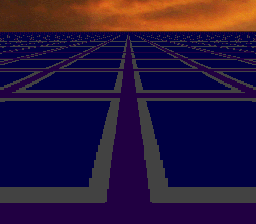
\includegraphics[height=4.5cm, width=\textwidth, keepaspectratio]{img/Mode_7.png}
    \label{fig:}
    \caption{Exemplo do Modo 7\cite{fonte_modo_7}}   
  \end{center}
\end{figure}

\section{O Áudio}

A unidade de processamento de áudio (APU) do console consiste de um co-processador Nintendo S-SMP, baseado no Sony SPC700 de 8bits, um Processador de Sinal Digital (DSP) de 16 bits, uma SRAM compartilhada de 64kB e uma boot ROM de 64 bytes.\\
O APU funciona com um clock de 24.576 MHz e só se comunica com a CPU via 4 registradores no "Bus B".\\
A RAM é acessada a 3.072 MHz, com os acessos multiplexados entre o SPC700 (1/3) e o DSP(2/3). Ela é utilizada para armazenar o programa e a pilha do SPC700, os dados da amostra e tabela de ponteiros de áudio e o buffer de eco do DSP.\\

O SPC700 aceita instruções e dados da CPU e manipula os registros do DSP para gerar a música e os efeitos sonoros. O DSP gera uma onda de 16 bits a 32kHz mixando a entrada de 8 vozes independentes e um filtro FIR de ordem 8 normalmente usado para reverberação. Cada voz pode tocar sua amostra a uma taxa variável, com Interpolação Gaussiana, "stereo panning" e envelopagem ADSR, linear, não-linear ou direta. Todas as amostras de áudio são comprimidas utilizando um tipo de modulação ADPCM chamada de Bit-rate reduction (BRR).\\

Como o sistema de áudio é praticamente independente, o estado do sistema pode ser conectado ou emulado em um computador hospedeiro. Sua saída pode ser salva como um formato .SPC e tal formato pode ser executado de maneira independente, com exceção à alguns jogos que constantemente utilizam amostras da ROM.\cite{AnomieDSPDoc}\cite{AnomieSPC700Doc}\cite{ApuManual}\\

\begin{figure}[h!]
	\centering
    \includegraphics[width=0.7\textwidth]{img/291px-S-SMP_01.jpg}
\end{figure}

\section{O Cartucho}
Os conectores do cartucho podiam ser serparados em 5 categorias:\\
\begin{itemize}
\item conectores da ROM;
\item conectores DSP;
\item conectorres MAD-1;
\item conectores CIC;
\item conectores SRAM.
\end{itemize}
\begin{figure}[h!]
	\centering
    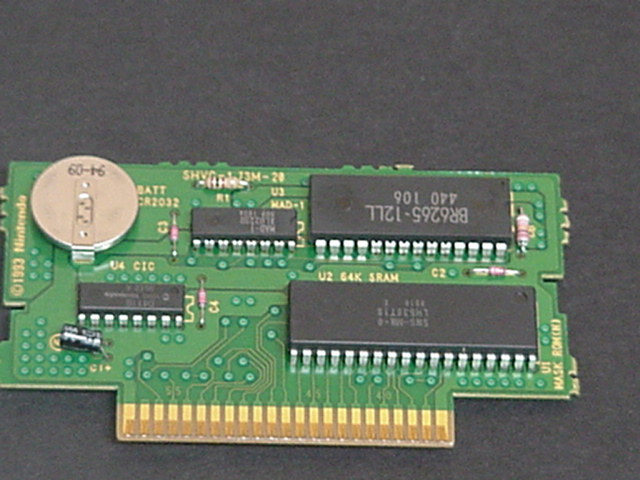
\includegraphics[width=0.7\textwidth]{img/cart0}
    \caption{Circuito de um cartucho}
\end{figure}
\subsection*{Tabela dos conectores}

\begin{tabular}{rlrl}
21.477MHz Clock  & 01  & 32  & /WRAM\\
EXPAND  & 02  & 33  & REFRESH\\
PA6  & 03  & 34  & PA7  \\
/PARD  & 04  & 35  & /PAWR\\
&     &     &      \\
GND  & 05  & 36  & GND  \\
A11  & 06  & 37  & A12  \\
A10  & 07  & 38  & A13  \\
A9  & 08  & 39  & A14  \\
A8  & 09  & 40  & A15  \\
A7  & 10  & 41  & BA0  \\
A6  & 11  & 42  & BA1  \\
A5  & 12  & 43  & BA2  \\
A4  & 13  & 44  & BA3  \\
A3  & 14  & 45  & BA4  \\
A2  & 15  & 46  & BA5  \\
A1  & 16  & 47  & BA6  \\
A0  & 17  & 48  & BA7  \\
/IRQ  & 18  & 49  & /CART\\
D0  & 19  & 50  & D4   \\
D1  & 20  & 51  & D5   \\
D2  & 21  & 52  & D6   \\
D3  & 22  & 53  & D7   \\
/RD  & 23  & 54  & /WR  \\
CIC out data (p1)  & 24  & 55  & CIC out data (p2)\\
CIC  in data (p7)  & 25  & 56  & CIC in clock (p6)\\
/RESET  & 26  & 57  & CPU\_CLOCK\\
Vcc  & 27  & 58  & Vcc  \\
&     &     &      \\
PA0  & 28  & 59  & PA1  \\
PA2  & 29  & 60  & PA3  \\
PA4  & 30  & 61  & PA5  \\
Left Audio Input  & 31  & 62  & Right Audio Input\\

\end{tabular}
 
\subsection*{definições:}
A0-A15  - barramento de endereços A (offset)\\
BA0-BA7 - barramento de endereços A (bank)\\
/RD - linha de controle de leitura para o barramento de endereços A\\
/WR - linha de controle de escrita para o barramento de endereços A\\
/CART - coloca como baixa pelo decodificador de endereço do console quando barramento de endereços A está acessando memória na região do cartucho\\
/WRAM - coloca como baixa pelo decodificador de endereço do console quando barramento de endereços A está acessando memória na região WRAM\\
/IRQ - um cartucho pode requerer uma interrupção IRQ na CPU principal colocando esta como baixa\\
PA0-PA7 - barramento de endereços B\\
/PARD - linha de controle de leitura para o barramento de endereços B\\
/PAWR - linha de controle de escrita para o barramento de endereços B\\
CIC - chip de segurança\\
EXPAND - linha é mudada para alta através de um resistor, a única outra coisa conectada a este é um pino da porta de expansão\\
CPU\_CLOCK - dependendo da tempo de um ciclo da memória atual o clock da CPU pode ser alterado\\
REFRESH - sinal de refresh para a memória\\
Audio Inputs - entradas de áudio do console\\

\subsection*{Conectores da ROM}
Isto vale tanto para a versão PAL quanto NTSC(32 ou 36 pinos).\\

\begin{tabular}{rlrl}
               A17 &  01   &      32  & Vcc\\
               A18 &  02   &      31  & /OE\\
               A15 &  03   &      30  & A19\\
               A12 &  04   &      29  & A14\\
                A7 &  05   &      28  & A13\\
                A6 &  06   &      27  & A8\\
                A5 &  07   &      26  & A9\\
                A4 &  08   &      25  & A11\\
                A3 &  09   &      24  & A16\\
                A2 &  10   &      23  & A10\\
                A1 &  11   &      22  & /CS\\
                A0 &  12   &      21  & D7\\
                D0 &  13   &      20  & D6\\
                D1 &  14   &      19  & D5\\
                D2 &  15   &      18  & D4\\
               Vss &  16   &      17  & D3\\

\end{tabular}\\
ou\\

\begin{tabular}{rlrl}
               A20  & 01     &    36  & Vcc\\
               A21  & 02     &    35  & A22\\
               A17  & 03     &    34  & Vcc\\
               A18  & 04     &    33  & /OE\\
               A15  & 05     &    32  & A19\\
               A12  & 06     &    31  & A14\\
                A7  & 07     &    30  & A13\\
                A6  & 08     &    29  & A8\\
                A5  & 09     &    28  & A9\\
                A4  & 10     &    27  & A11\\
                A3  & 11     &    26  & A16\\
                A2  & 12     &    25  & A10\\
                A1  & 13     &    24  & /CS\\
                A0  & 14     &    23  & D7\\
                D0  & 15     &    22  & D6\\
                D1  & 16     &    21  & D5\\
                D2  & 17     &    20 &  D4\\
               Vss  & 18     &    19 &  D3\\
\end{tabular}



\subsection*{Conectores DSP}

É assim que a maioria dos chips DSP são conectados.\\

\begin{tabular}{rlrl}
               Vcc &  01  & 28  & Vcc\\
               Vcc &  02  & 27  & register select\\
                nc &  03  & 26  & /CS \\
                nc &  04  & 25  & /RD\\
                nc &  05  & 24  & /WR\\
                D0 &  06  & 23  & nc\\
                D1 &  07  & 22  & nc\\
                D2 &  08  & 21  & Vcc\\
                D3 &  09  & 20  & Vcc\\
                D4 &  10  & 19  & Vcc\\
                D5 &  11  & 18  & Vcc\\
                D6 &  12  & 17  & GND\\
                D7 &  13  & 16  & RESET\\
                D8 &  14  & 15  & CLOCK\\
\end{tabular}


\subsection*{Conectores MAD-1}

MAD-1 significa "Memory Address Decoder revision 1",  decodificador de endereço de memória, revisão 1. É usado para o mapeamento de memória em ambos HiRom e LoRom. E é usado para o controle da energia da bateria na RAM estática.\\

O chip MAD-1:\\
\begin{tabular}{rlrl}                
                                /HI & 01   &   16 & /LOW\\
                           SRAM /CS & 02   &   15 & A15 (LoRom), A13 (HiRom) \\
                                 NC & 03   &   14 & BA4 (LoRom), A14 (HiRom) \\
                            ROM /OE & 04   &   13 & BA5 \\
                           SRAM Vcc & 05   &   12 & Vcc ou BA6 (LoRom), A15 ou BA6(HiRom)... \\
                                Vcc & 06   &   11 & /CART (pad 49 na interface do cartucho) \\
         resistor to +3V of battery & 07   &   10 & GND=LoRom, Vcc=HiRom \\
                                GND & 08   &   09 & /RESET (pad 26 na interface do cartucho) \\
\end{tabular}
 
 
/HI --- se dois ROM chips, este seleciona o superiore.\\
/LOW --- se dois ROM chips, este seleciona o inferior. 

\subsection*{Chip de Segurança}

No chip marcado com: D411;\\
na placa marcada com: CIC.\\

\begin{tabular}{rlrl}
            pad24 & 01   &   16 & Vcc\\
            pad55 & 02   &   15 & NC\\
               NC & 03   &   14 & NC\\
              GND & 04   &   13 & NC\\
               NC & 05   &   12 & NC\\
            pad56 & 06   &   11 & NC\\
            pad25 & 07   &   10 & NC\\
              GND & 08   &   09 & NC\\
\end{tabular}


\subsection*{Conectores SRAM}

A SRAM de 16kbit usada pela nintendo\\
\begin{tabular}{rlrl}
                A7 &  01   &      24  & Vcc\\
                A6 &  02   &      23  & A8\\
                A5 &  03   &      22  & A9\\
                A4 &  04   &      21  & /WE\\
                A3 &  05   &      20  & /OE\\
                A2 &  06   &      19  & A10\\
                A1 &  07   &      18  & /CS\\
                A0 &  08   &      17  & D7\\
                D0 &  09   &      16  & D6\\
                D1 &  10   &      15  & D5\\
                D2 &  11   &      14  & D4\\
               Vss &  12   &      13  & D3\\
\end{tabular}

A SRAM de 256kbit usada pela Nintendo\\
(HY62256ALLP-10 em MarioPaint)\\
\begin{tabular}{rlrl}
               A14  & 01   &      28 &  Vcc\\
               A12  & 02   &      27 &  /WE\\
                A7  & 03   &      26 &  A13\\
                A6  & 04   &      25 &  A8\\
                A5  & 05   &      24 &  A9\\
                A4  & 06   &      23 &  A11\\
                A3  & 07   &      22 &  /OE\\
                A2  & 08   &      21 &  A10\\
                A1  & 09   &      20 &  /CS\\
                A0  & 10   &      19 &  D7\\
                D0  & 11   &      18 &  D6\\
                D1  & 12   &      17 &  D5\\
                D2  & 13   &      16 &  D4\\
               GND  & 14   &      15 &  D3\\
\end{tabular}
  \subsection{Enhancement Chips}
  \begin{figure}[h!]
  	\centering
      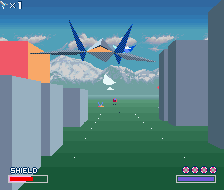
\includegraphics[width=0.7\textwidth]{img/starfox}
      \caption{Star Fox, que usa o chip Super FX}
  \end{figure}
  Como parte de todo um plano o SNES, ao invés de incluir uma CPU cara que ficaria obseleta em poucos anos, os designers de hardware facilitaram a interface para chips coprocessadores para o console. Isto é caracterizado pela adição de 16 pinos extras no cartucho.\\
  O Super FX é um RISC CPU desenhado para realizar funções que a CPU principal não seria capaz de realizar. O chip era primariamente usado para criar jogos 3D com poligonos, mapas de texturas e sombra de fontes de luz. O chip podia também ser usado para melhorar jogos 2D.\\
  O chip processador de sinais digitais de ponto fixo da Nintendo (DSP) permitia calculos rápidos baseados em vetores, conversões de bitmap, ambas transformações de coordenadas 2D e 3D, e outras funções. Quatro revisões do chip existem, cada um fisicamente idêntico com diferentes microcodes. A versão DSP-1, incluindo as posteriores correções de bug 1A e 1B foram as mais usadas; o DSP-2, DSP-3 e DSP-4 foram usadas em apenas 1 título cada.\\
  Similar ao CPU 5A22 do console, o chip SA-1 contem um núcleo 65c816 com clock de 10 MHz, um mapeador de memória, DMA, decompressão e conversão de bitplane por circuito, muitos timers programáveis, e a funcionalidade CIC.\\
No Japão, jogos podiam ser baixados gratuitamente nos quiosques Nintendo Powere em cartuchos especiais contendo memórias flash e um chip MegaChips MX15001TFC. O chip gerenciava a comunicação com o quiosque para baixar a imagem da ROM, e prover um menu inicial para selecionar qual jogo seria jogado. Alguns títulos eram disponíveis ambos em cartucho e em download, enquanto outros eram apenas na forma de download. O serviço acabou em 2007.\\
  Muitos cartuchos continham outros chip de expansão, a maioria dos quais foram criados para uso por uma única companhia em poucos títulos.

\section{Checking Integrated Circuit(CIC) e Pirataria}
\subsection*{regional lockout}
\begin{figure}[h!]
	\centering
    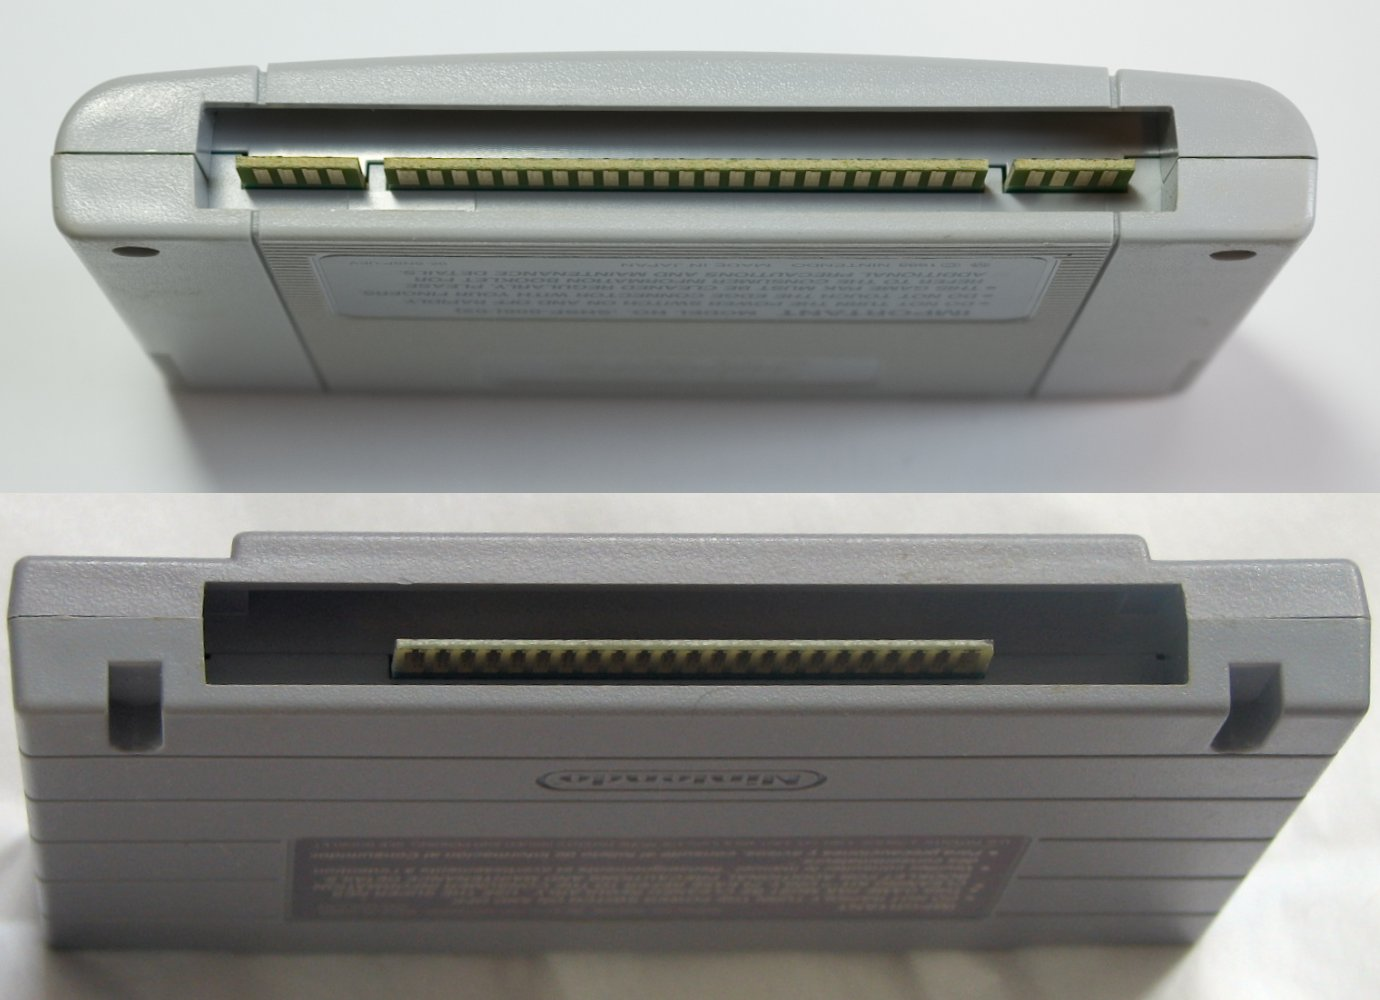
\includegraphics[width=0.7\textwidth]{img/snescartcomp}
    \label{fig:comparative}
    \caption{Comparativo de cartuchos SNES em versões PAL e NTSC, respectivamente}
\end{figure}
A primeira forma que a Nintendo criou para proteger o uso indevido foi limitando o uso do cartucho por região, a limitação incluía incompatibilidade tanto física quanto de Hardware.\\
Físicamente os Cartuchos de região PAL eram diferentes dos de regiões NTSC, como pode ser visto na figura \ref{fig:comparative}, essa incompatibilidade era facilmente superada com adaptadores ou por modificação do console.\\
\subsection*{CIC}
No hardware, a Nintendo incluiu em seu vídeo-game um aprimoramento do sistema existente no NES, o CIC. No NES quem conseguiu burlar este sistema primeiro foi a Atari.\\
O sistema era composto de duas partes, um microcontrolador no console que checa o cartucho inserido para autenticação e um chip "chave" no cartucho que responde o código sob demanda. Se o cartucho não fornece a autenticação o chip CIC poderia resetar a CPU em todo cicli, até que um chip autorizado fosse colocado. O reinicio constante da CPU impedia a inicialização do sistema.\\
O sistema era burlado clonando o chip de verificação, tornando desnecessário um desbloqueio físico do console.
\begin{figure}[h!]
	\centering
    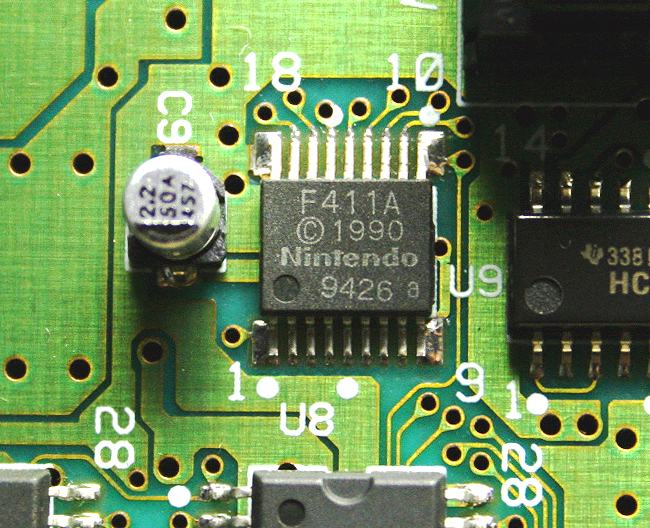
\includegraphics[width=0.7\textwidth]{img/snescicvg}
    \caption{Chip CIC do SNES no Vídeo Game}
\end{figure}
\begin{figure}[h!]
	\centering
    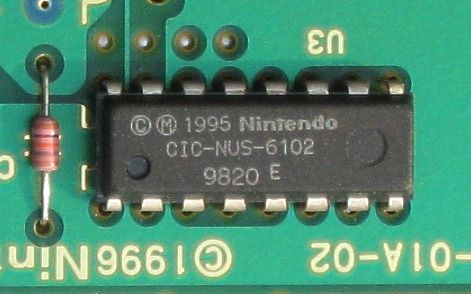
\includegraphics[width=0.7\textwidth]{img/snesciccart}
    \caption{Chip CIC dos Cartuchos do SNES}
\end{figure}
%\section{Emulação}

\section{O Gamepad}
\begin{tabular}{ccc}
Pin	& Description	& Wire Color\\
\hline 1 & +5v	& White\\
2 & Data Clock &Yellow\\
3 & Data Latch & Orange\\
4 & Serial Data	& Red\\
5 & N/C & -\\
6 & N/C & -\\
7 & Ground & Brown\\
\end{tabular}\\

Notas traduzidas e adaptadas do texto de Jim Christy\cite{jimc}:\\

Conectores 5 e 6 mostram uma voltagem de 5v em um DMM.\\
Apesar da discos de borracha setem usados para prover resposta tatil dos botões eles não são capacitivos, mas carbono impregnado na borracha criar um caminho resistivo de 200 ohms atraves de 2 PCB revestidos de carbono que encostam quando precionados.\\
\begin{figure}[h!]
	\centering
    \includegraphics[width=0.7\textwidth]{img/snescontrol}
    \caption{Gamepads do SNES, versão japonesa e americana, respectivamente}
\end{figure}
A cada 16.67ms (ou aproximadamente 60Hz), A CPU do SNES envia uma mensagem de 12us de largura, dado positivo indo para o pino 3. Esta instrui os ICs no controle a verificar o estado de todos os botões internamente. Seis microsegundos depois de chegar o pulso, o CPU envia 16 pulsos no pin 2. Estes são responsáveis por 50\% do tempo total do ciclo. Os controles seriais o estado do botão pressionado para o pino 4 a cada ciclo.\\
Cada botão do controle é atribuído a um ID específico, que corresponde ao clock do ciclo durante o qual o botão será reportado. A tabela abaixo lista os ids de todos os botões. Note que multiplos butões podem ser pressionados ao mesmo tempo. Também note que uma lógica "alta" na linha de dados serial representa que nenhum botão fora precionado.\\
No fim da sequencia de 16 cíclos a linha de dados serial é reduzida até o próximo pulso. A única forma de desviar deste protocoloé aparentemente no primeiro ciclo. Pelo clock ser normalmente alto, a primeira transição que é feita logo depois do pulso inicial é uma transição de baixo para cima. Como os dados para o primeiro butão serão atravessados nesta transição, os dados serão dirigidos antecipadamente. Os controles do SNES dirigem dados para o primero botão, caindo na beira da escala. Dados para todos os botões são digidos para todos os botões na subida do clock.\\
Lista de ids assinalados aos botões do controle.\\
\begin{tabular}{cc}
\label{tab:but}	
Clock & Cycle	Button Reported \\
1 &	B\\
2 &	Y\\
3 &	Select\\
4 &	Start\\
5 &	cima no joypad\\
6 &	baixo no joypad\\
7 &	esquerda no joypad\\
8 &	direita no joypad\\
9 &	A\\
10 &	X\\
11 &	L\\
12 &	R\\
13-16 &	nenhum (sempre alto)\\
\end{tabular}

Clock cycles 13-16 são essencialmente inutilizados. Seria interessante ver como o SNES reagiria a resposta nestes tempos. 

\section{Mão na Massa}

Para botar em prática o que aprendemos durante toda a pesquisa sobre o SNES. Nos demos o seguinte desafio: \textit{Construir um jogo que ao receber uma entrada do controle, mudasse a cor de fundo da tela.}\\
De início procuramos por frameworks de programação e acabamos descobrindo que a maioria da programação é feita diretamente em código Assembly. Descobrimos que a própria programação da trilha sonora era feita em Assembly e HEX para aumentar a eficiência do código.\cite{DaveWiseInterview}\\

Assim, começamos a entender como códigos simples funcionavam e, buscando na ótima fonte \textit{http://wiki.superfamicom.org/snes/show/HomePage}, encontramos vários tutoriais que facilitavam o árduo trabalho de juntar todas as peças e montar uma ROM funcional.

No primeiro passo baixamos um Assembler e um Linker e os instalamos.\cite{Tut1} Depois, utilizamos um código pronto para inicializar o SNES\cite{Tut2} e em seguida conseguimos criar uma ROM que alterava a cor de fundo da tela.\cite{Tut3}\\

Agora precisávamos conseguir ler a entrada do controlador\cite{Tut4} para depois construirmos a lógica que alteraria a cor da tela ao comando do botão. Aqui encontramos um grande obstáculo. A leitura do controle é muito complexa e sempre que parecia tudo certo, alguma coisa faltava e, sem a ajuda de um debugger ou de outras ferramentas, não conseguimos terminar o código que utilizava a entrada do teclado.\\

Assim, preferimos utilizar o código de outro tutorial\cite{Tut5} para entendermos o funcionamento não só da entrada do Joypad mas também da utilização de sprites e cores.

Além dessa parte de programação, encontramos dentre os documentos do site\\ \textit{www.romhacking.net} o código fonte completo da trilha sonora do jogo Top Gear.\cite{TopGear} Assim, também pudemos ver exemplos de código para o SPC700 e ter uma idéia de como era feita a programação do áudio de um jogo.


\section{Conclusão}

Durante toda a fase de pesquisa e, principalmente, na hora de montarmos uma ROM, percebemos que o SNES é muito mais complexo do que imaginávamos e, em conjunto com a escassez de documentos oficiais, exige um conhecimento técnico extremamente específico para ser programado.\\

Percebemos que essa escassez de documentação vem sendo melhorada apenas nos últimos anos, com a criação de websites com o intuito de agrupar e melhorar os documentos espalhados pela web, nenhum deles publicado pela própria Nintendo. Além disso, devido ao caráter amador da documentação, existem várias lacunas e vários pontos extensamente estudados, pois esses documentos seguem as vontades e necessidades de alguns poucos programadores, em sua maioria líderes de projetos de emulação.\\

Buscar, agrupar e utilizar essa documentação escassa foi um aprendizado muito grande. Apesar de ser um pouco desesperador saber exatamente o que cada bit de um certo registrador significa, mas não encontrar tutoriais para criar uma ROM simples, isso nos mostrou como funciona a comunidade do ROM Hacking e o alto conhecimento técnico desses programadores.\\

Foi uma pena notarmos que toda a documentação foi feita usando engenharia reversa e que a Nintendo não faz questão alguma de publicar seus arquivos fonte para alimentar esse cenário. Inclusive, um dos mais importantes desses programadores, byuu, dedica-se agora a criar um emulador cujo objetivo é praticamente uma documentação em software do hardware original do Super Nintendo, não apenas criando a possibilidade de executar jogos em outras plataformas, mas sendo uma representação fiel, ciclo a ciclo, de um Super Nintendo original.\cite{byuu}\\

Por fim, nos sentimos extremamente satisfeitos em nos aprofundarmos na organização do Super Nintendo Entertainment System e, apesar de termos apenas arranhado a superfície, tivemos a oportunidade de aprender uma imensidão de coisas novas: desde a programação em Assembly de um micro-processador de 16 bits até o funcionamento da linha de varredura das TVs de tubo, passando por técnicas de modulação de áudio, controladores com realidade aumentada e vários outros componentes de um vídeo game da época.


\begin{thebibliography}{99} % Referências

\bibitem{gamespot1}
  \href{http://www.gamespot.com/articles/nintendo-to-end-famicom-and-super-famicom-production/1100-6029220/}{Nintendo to end Famicom and Super Famicom production}
\bibitem{65c815datasheet}
  \href{http://westerndesigncenter.com/wdc/documentation/w65c816s.pdf}{Datasheet completo do microprocessador em pdf.}
\bibitem{AnomieMemMap}
  \href{http://www.romhacking.net/documents/193/}{Anomie's SNES Memory Mapping Doc}
\bibitem{AnomieRegDoc}
  \href{http://www.romhacking.net/documents/196/}{Anomie’s Register Doc}
\bibitem{fonte_modo_7} 
  \href{http://en.wikipedia.org/wiki/File:Mode\_7\_Test-0000.png}{Figura "Modo 7"}
\bibitem{AnomieDSPDoc}
  \href{http://www.romhacking.net/documents/191/}{Anomie's S-DSP Doc}
\bibitem{AnomieSPC700Doc}
  \href{http://www.romhacking.net/documents/197/}{Anomie's SPC700 Doc}
\bibitem{ApuManual}
  \href{http://web.archive.org/web/20090106230547/http://www.alpha-ii.com/snesmusic/files/spc700\_apu\_manual.txt}{APU Manual}
\bibitem{DaveWiseInterview}
  \href{http://www.nintendojo.com/features/interviews/interview-david-wise}{Interview: David Wise}
\bibitem{Tut1}
  \href{http://wiki.superfamicom.org/snes/show/Setting+Up+a+Programming+Environment}{Tutorial: Setting Up a Programming Environment }
\bibitem{Tut2}
  \href{http://wiki.superfamicom.org/snes/show/Initializing+the+SNES}{Tutorial: Initializing the SNES}
\bibitem{Tut3}
  \href{http://wiki.superfamicom.org/snes/show/Writing+Your+First+SNES+Program}{Tutorial: Writing Your First SNES Program }
\bibitem{Tut4}
  \href{http://wiki.superfamicom.org/snes/show/Polling+Controller+Input}{Tutorial: Polling Controller Input }
\bibitem{Tut5}
  \href{http://wiki.superfamicom.org/snes/show/Making+a+Small+Game+-+Tic-Tac-Toe}{Tutorial: Making a Small Game - Tic-Tac-Toe }
\bibitem{TopGear}
  \href{http://www.romhacking.net/documents/589/}{Top Gear Music Source Code}
\bibitem{byuu}
  \href{http://byuu.org/snes/preservation/}{byuu's Homepage - Snes::Preservation}

\end{thebibliography}

\end{document}
